%!TEX root = ../main.tex
\begin{frame}{Reproductive number}
    \setlength{\leftmargini}{1mm}
    \begin{textblock*}{65mm}(0mm, 25mm)
        \only<1>{
            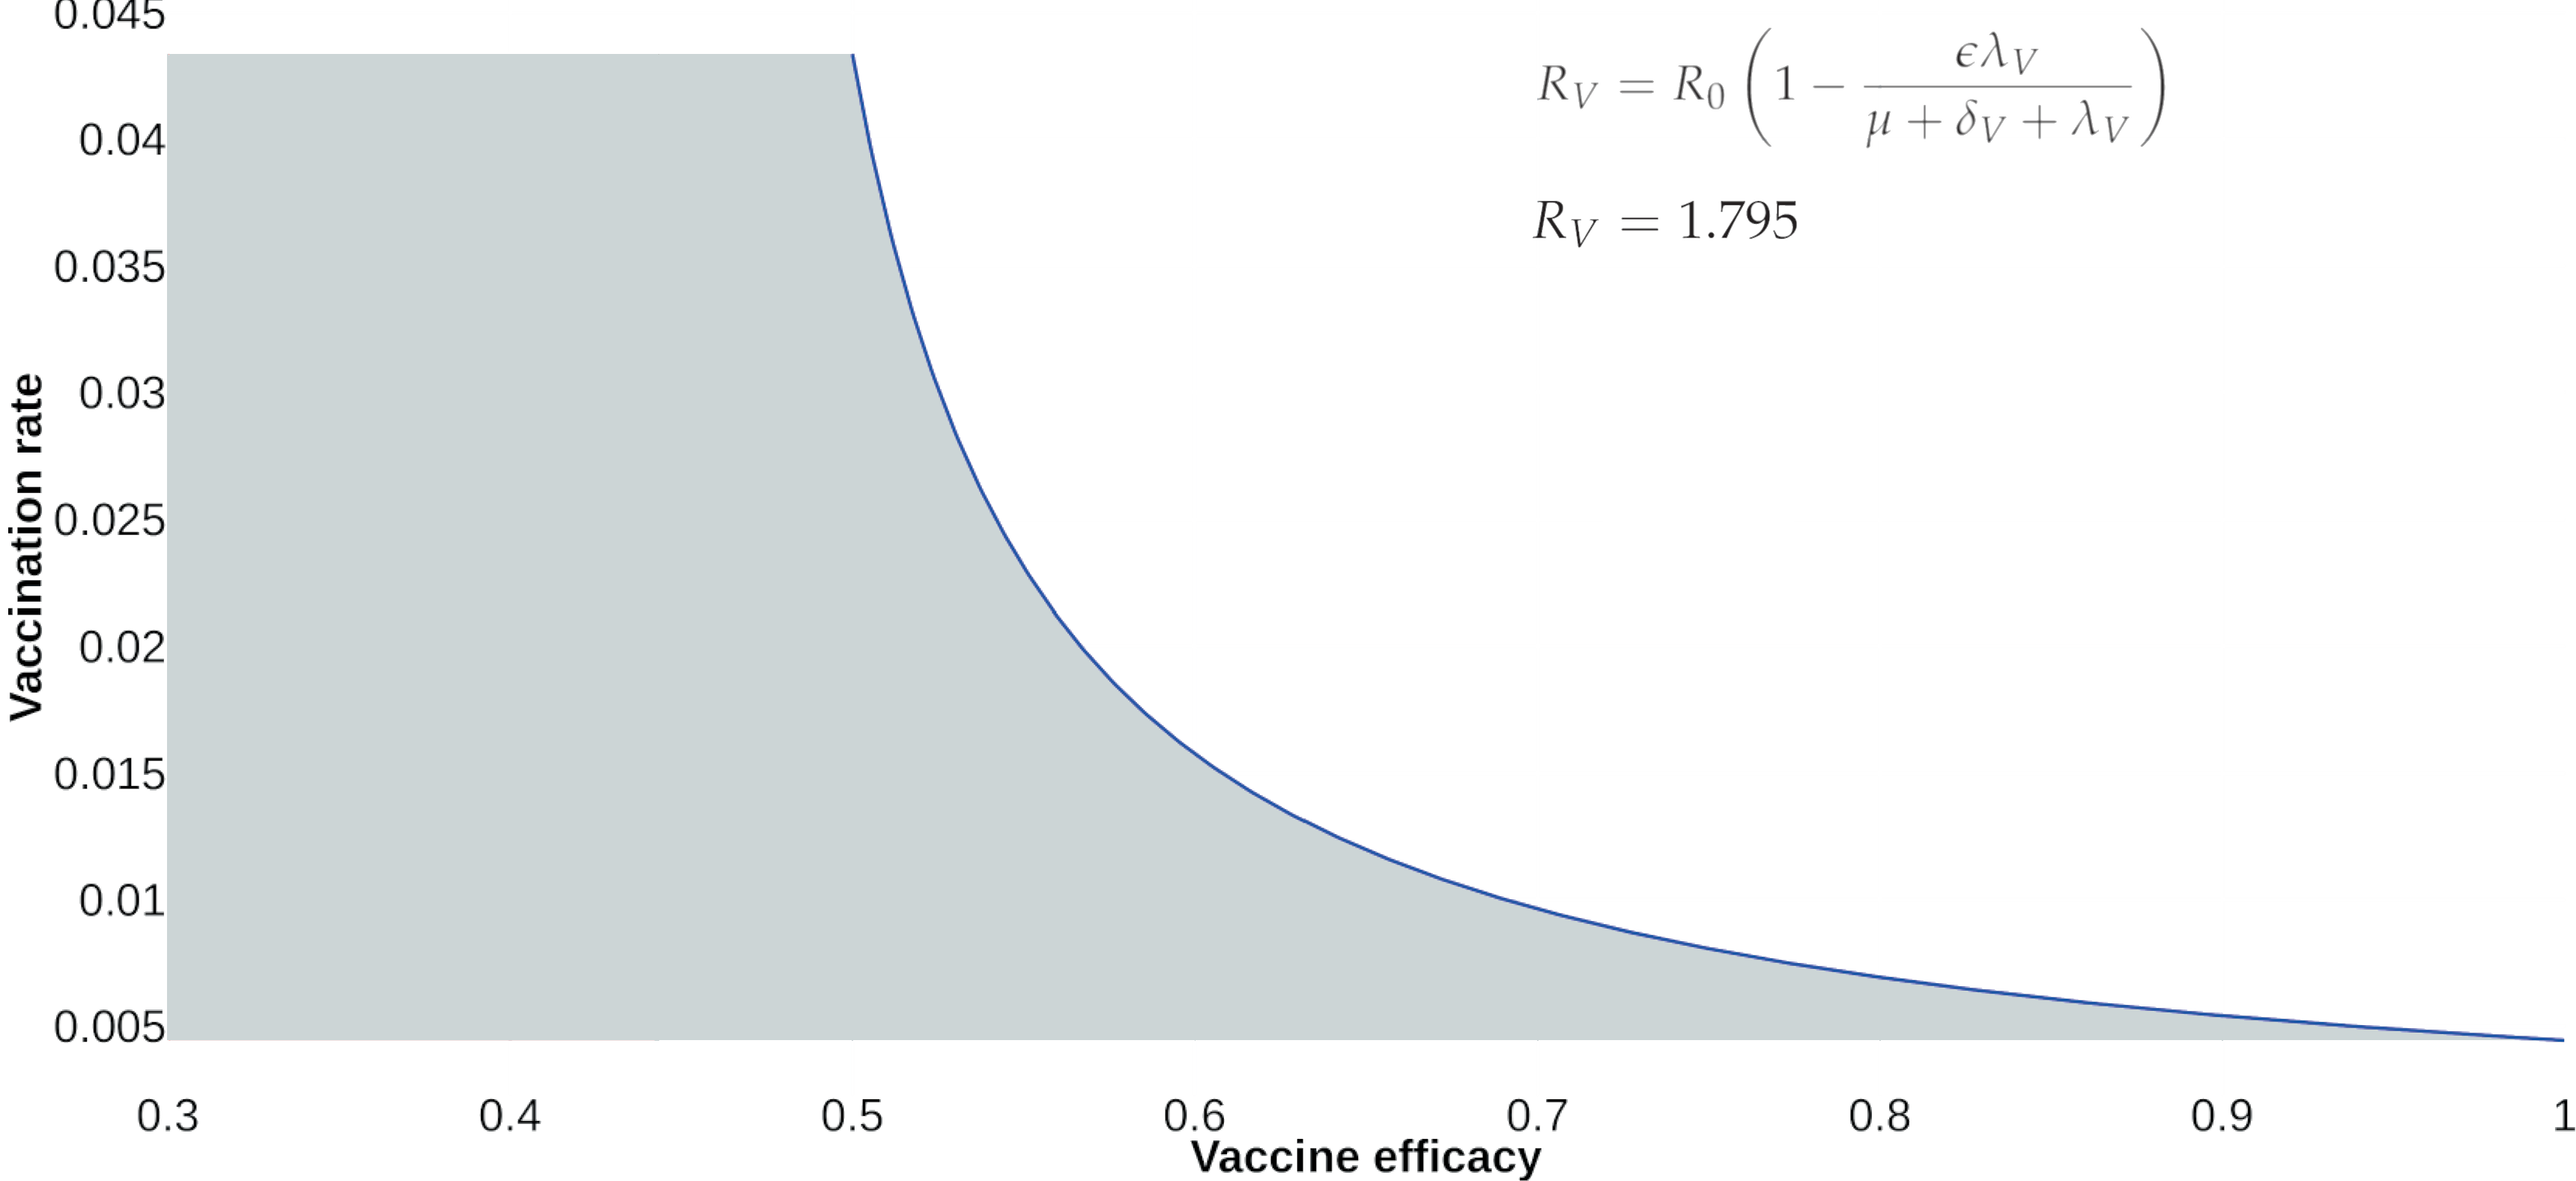
\includegraphics[scale=.875,%
                keepaspectratio]{assets/RvAnimation//r_zero_vac_efficiency01.png}
        }
        \only<2>{
            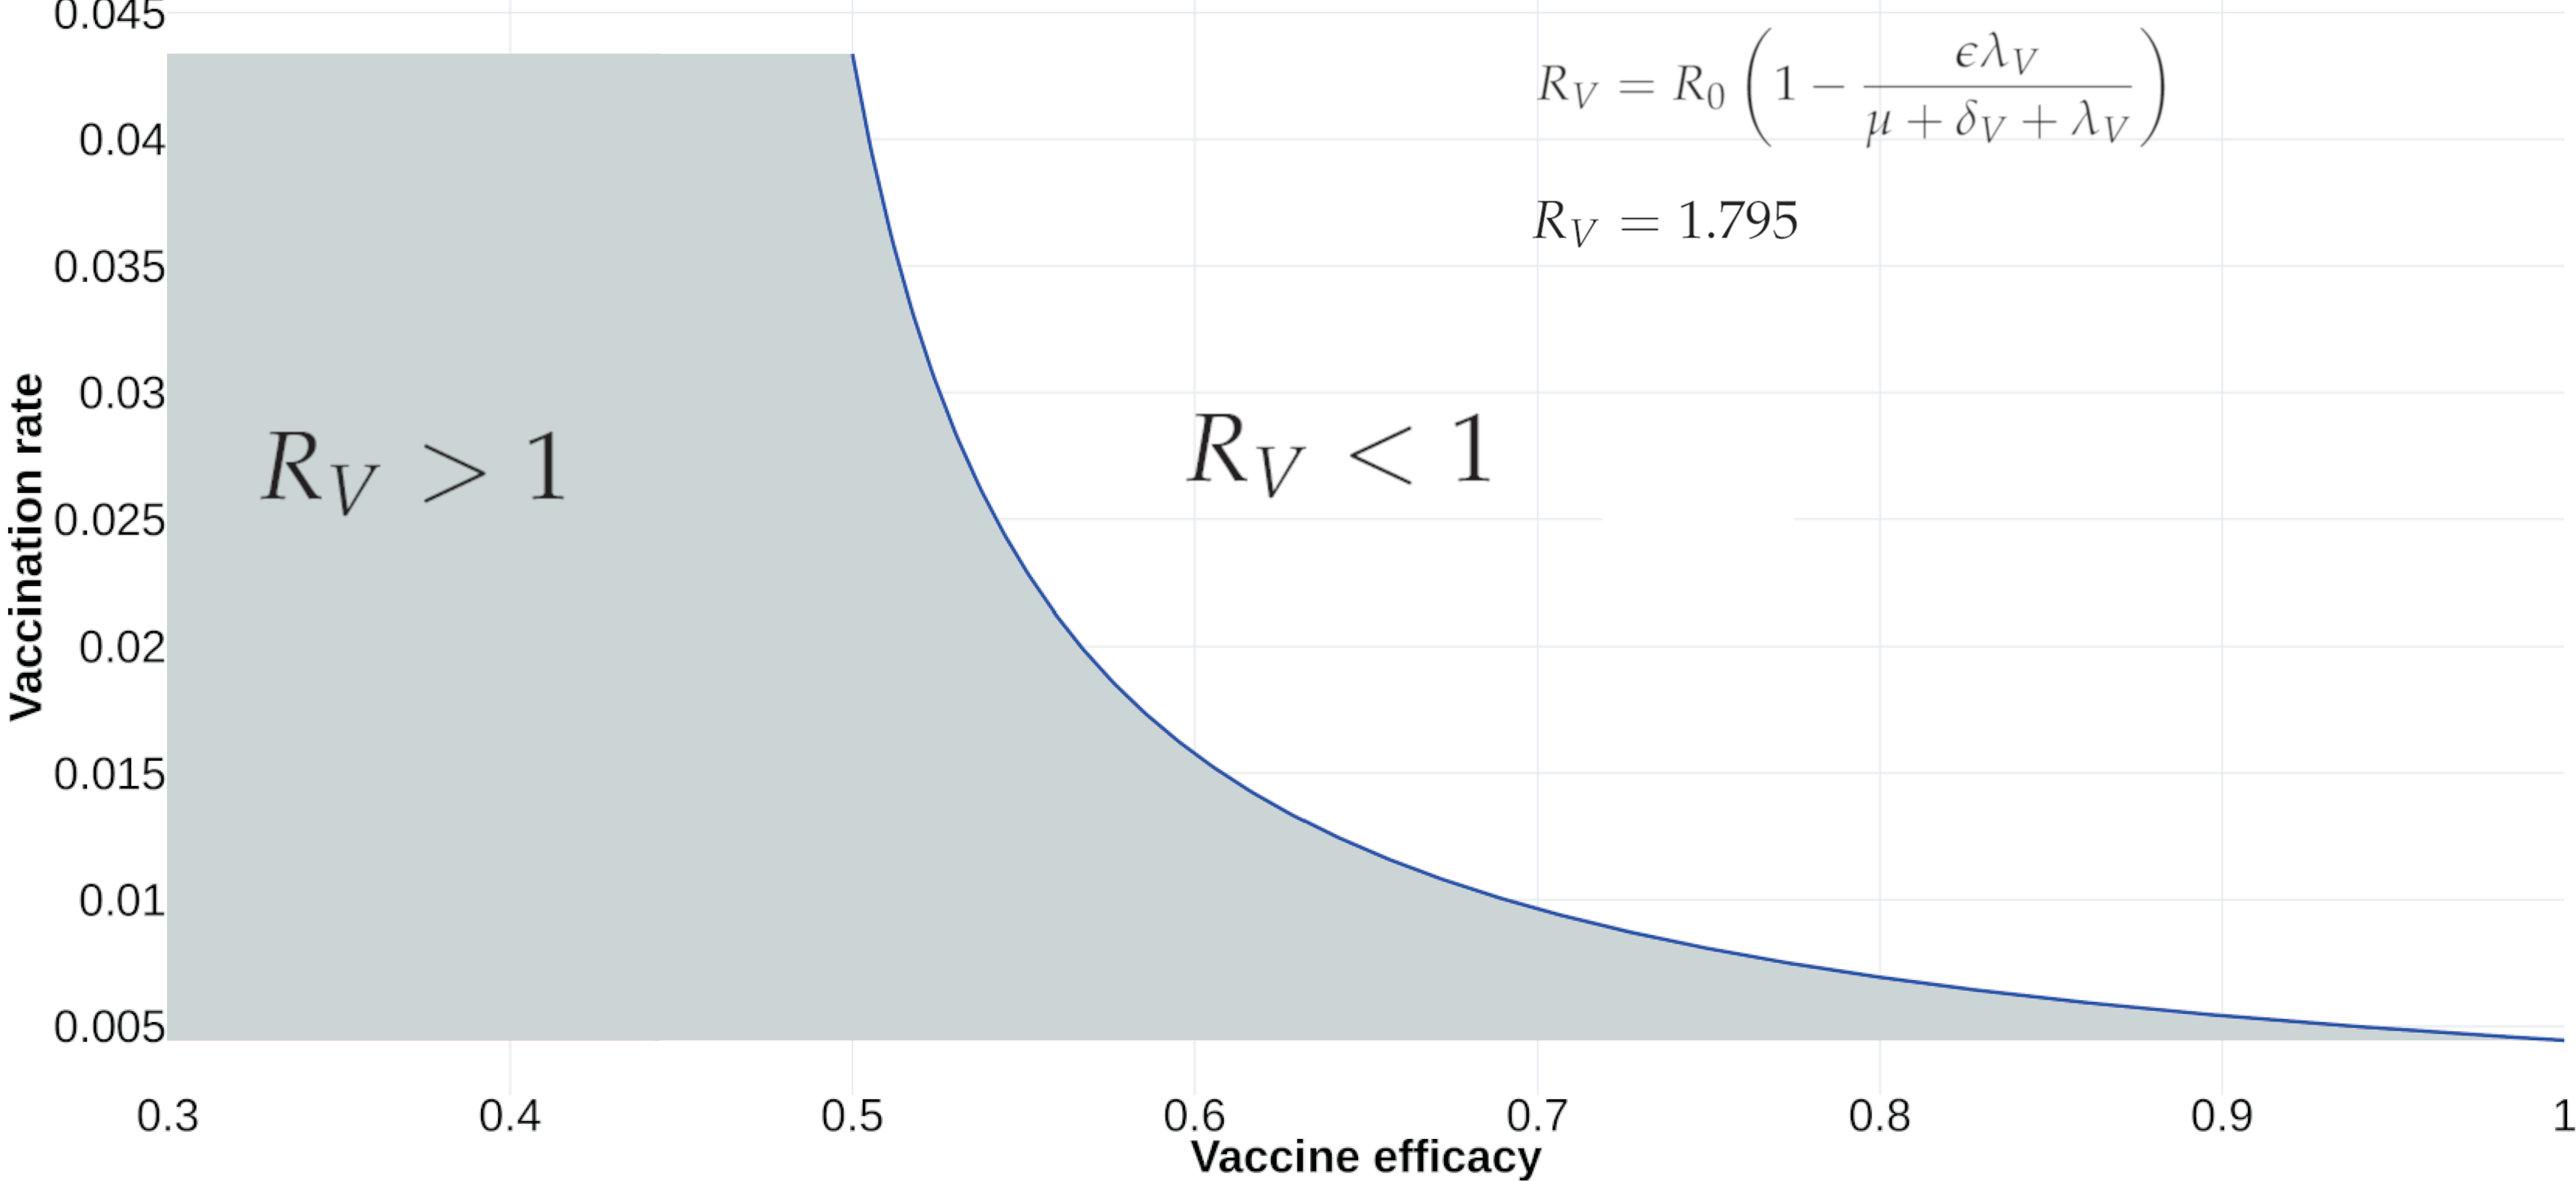
\includegraphics[scale=.875,%
            keepaspectratio]{assets/RvAnimation//r_zero_vac_efficiency02.png}
        }
        \only<3>{
            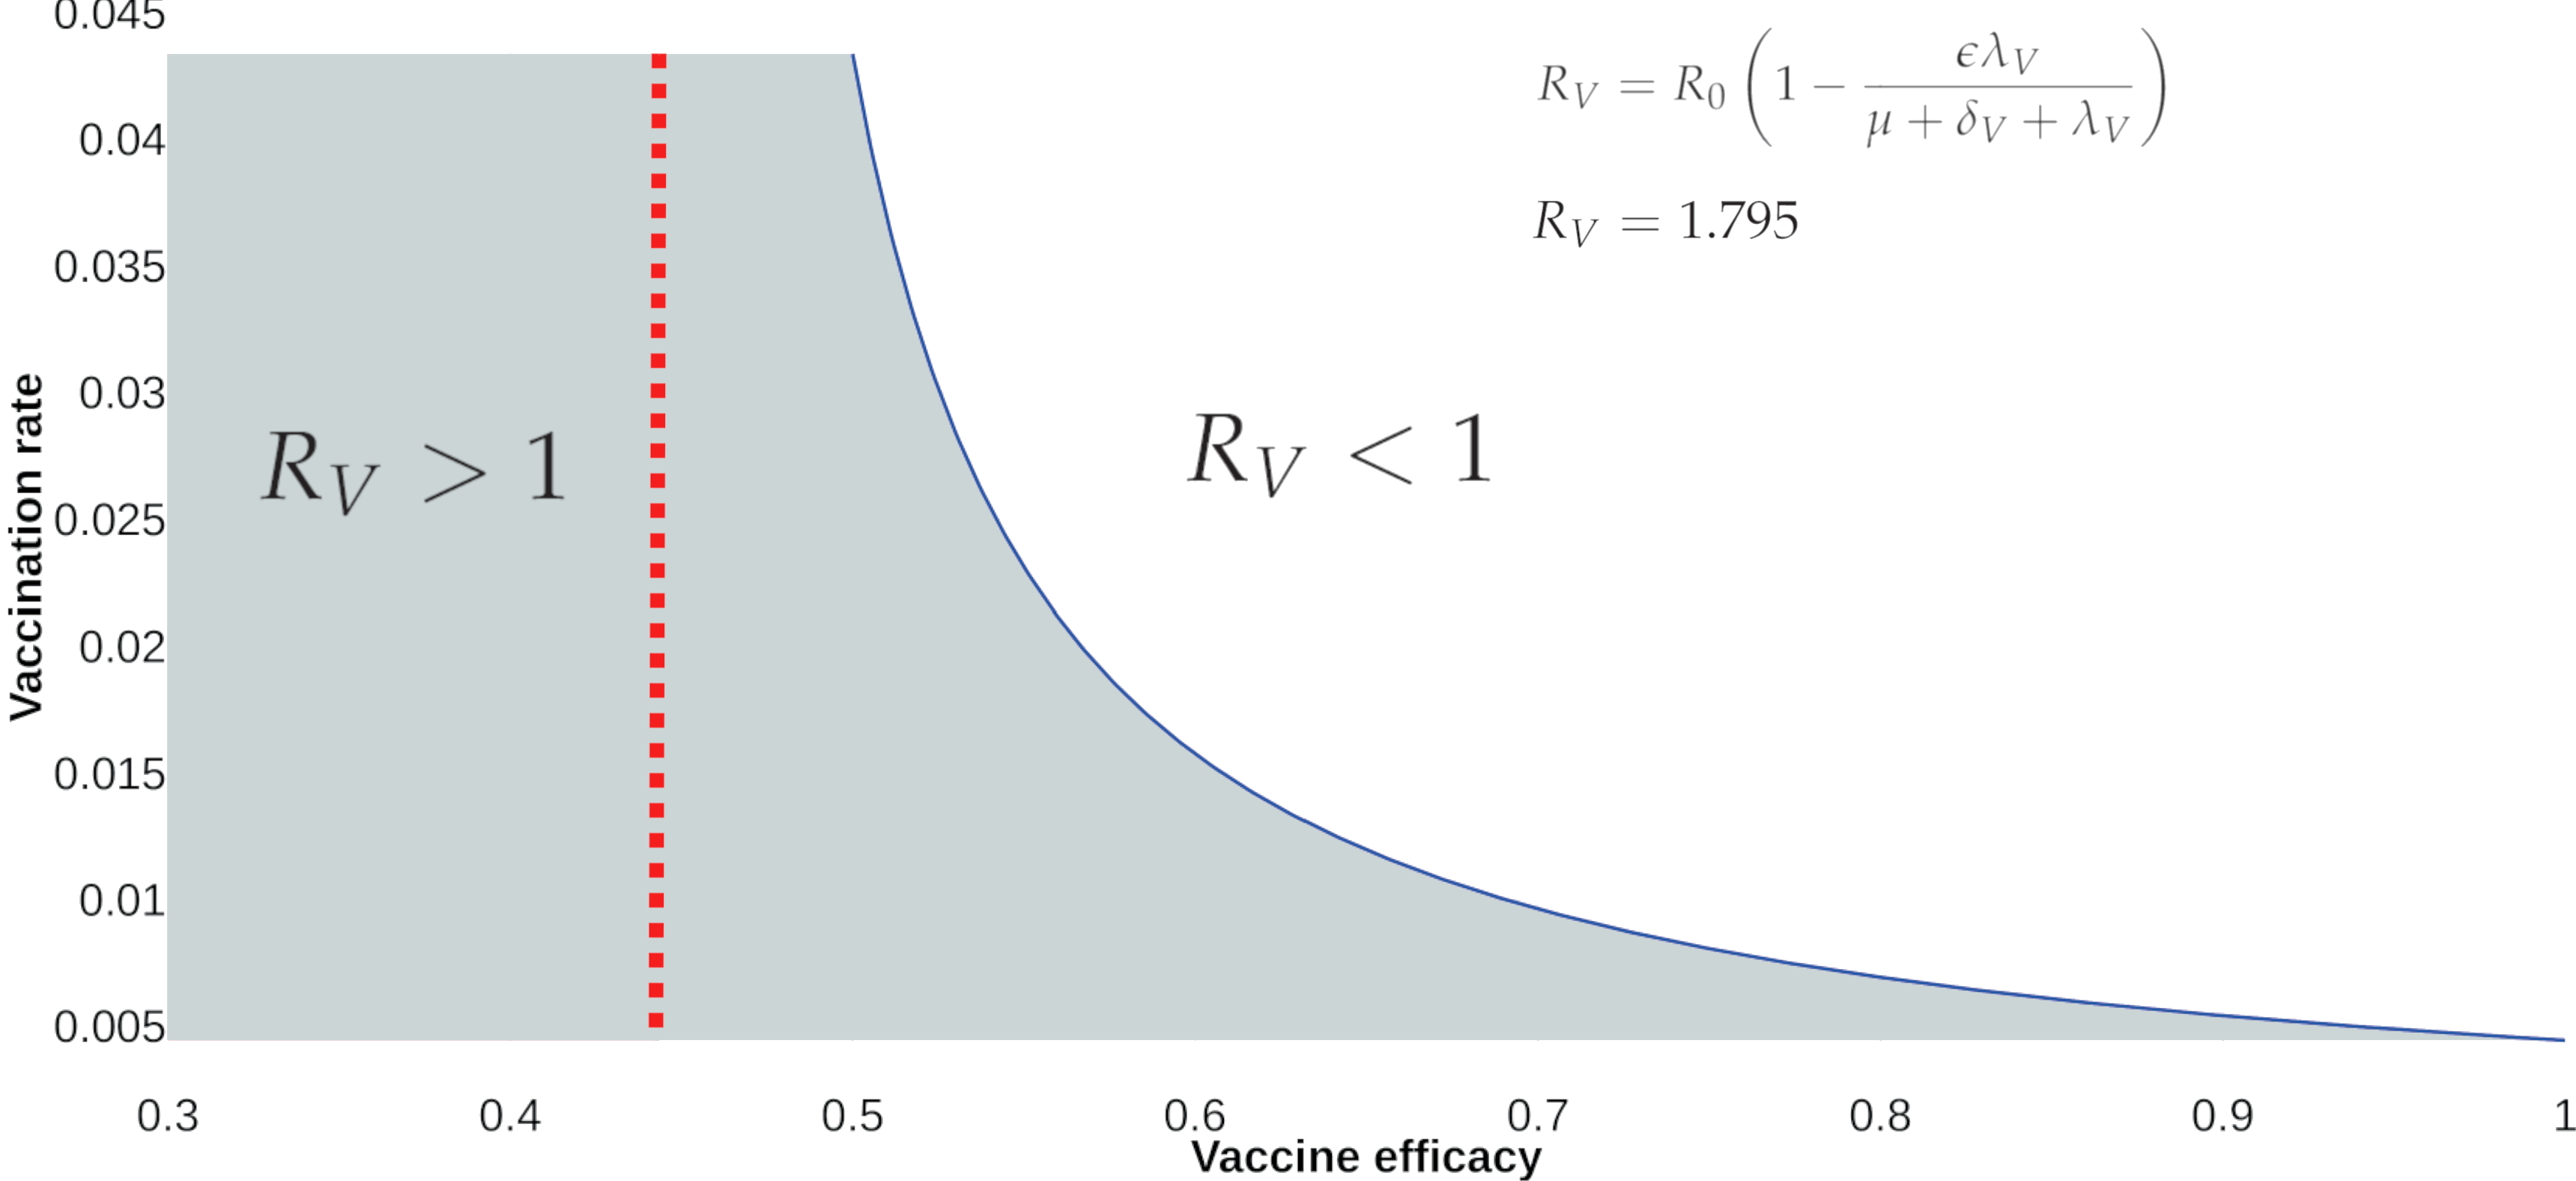
\includegraphics[scale=.875,%
            keepaspectratio]{assets/RvAnimation//r_zero_vac_efficiency03.png}
        }
        \only<4>{
            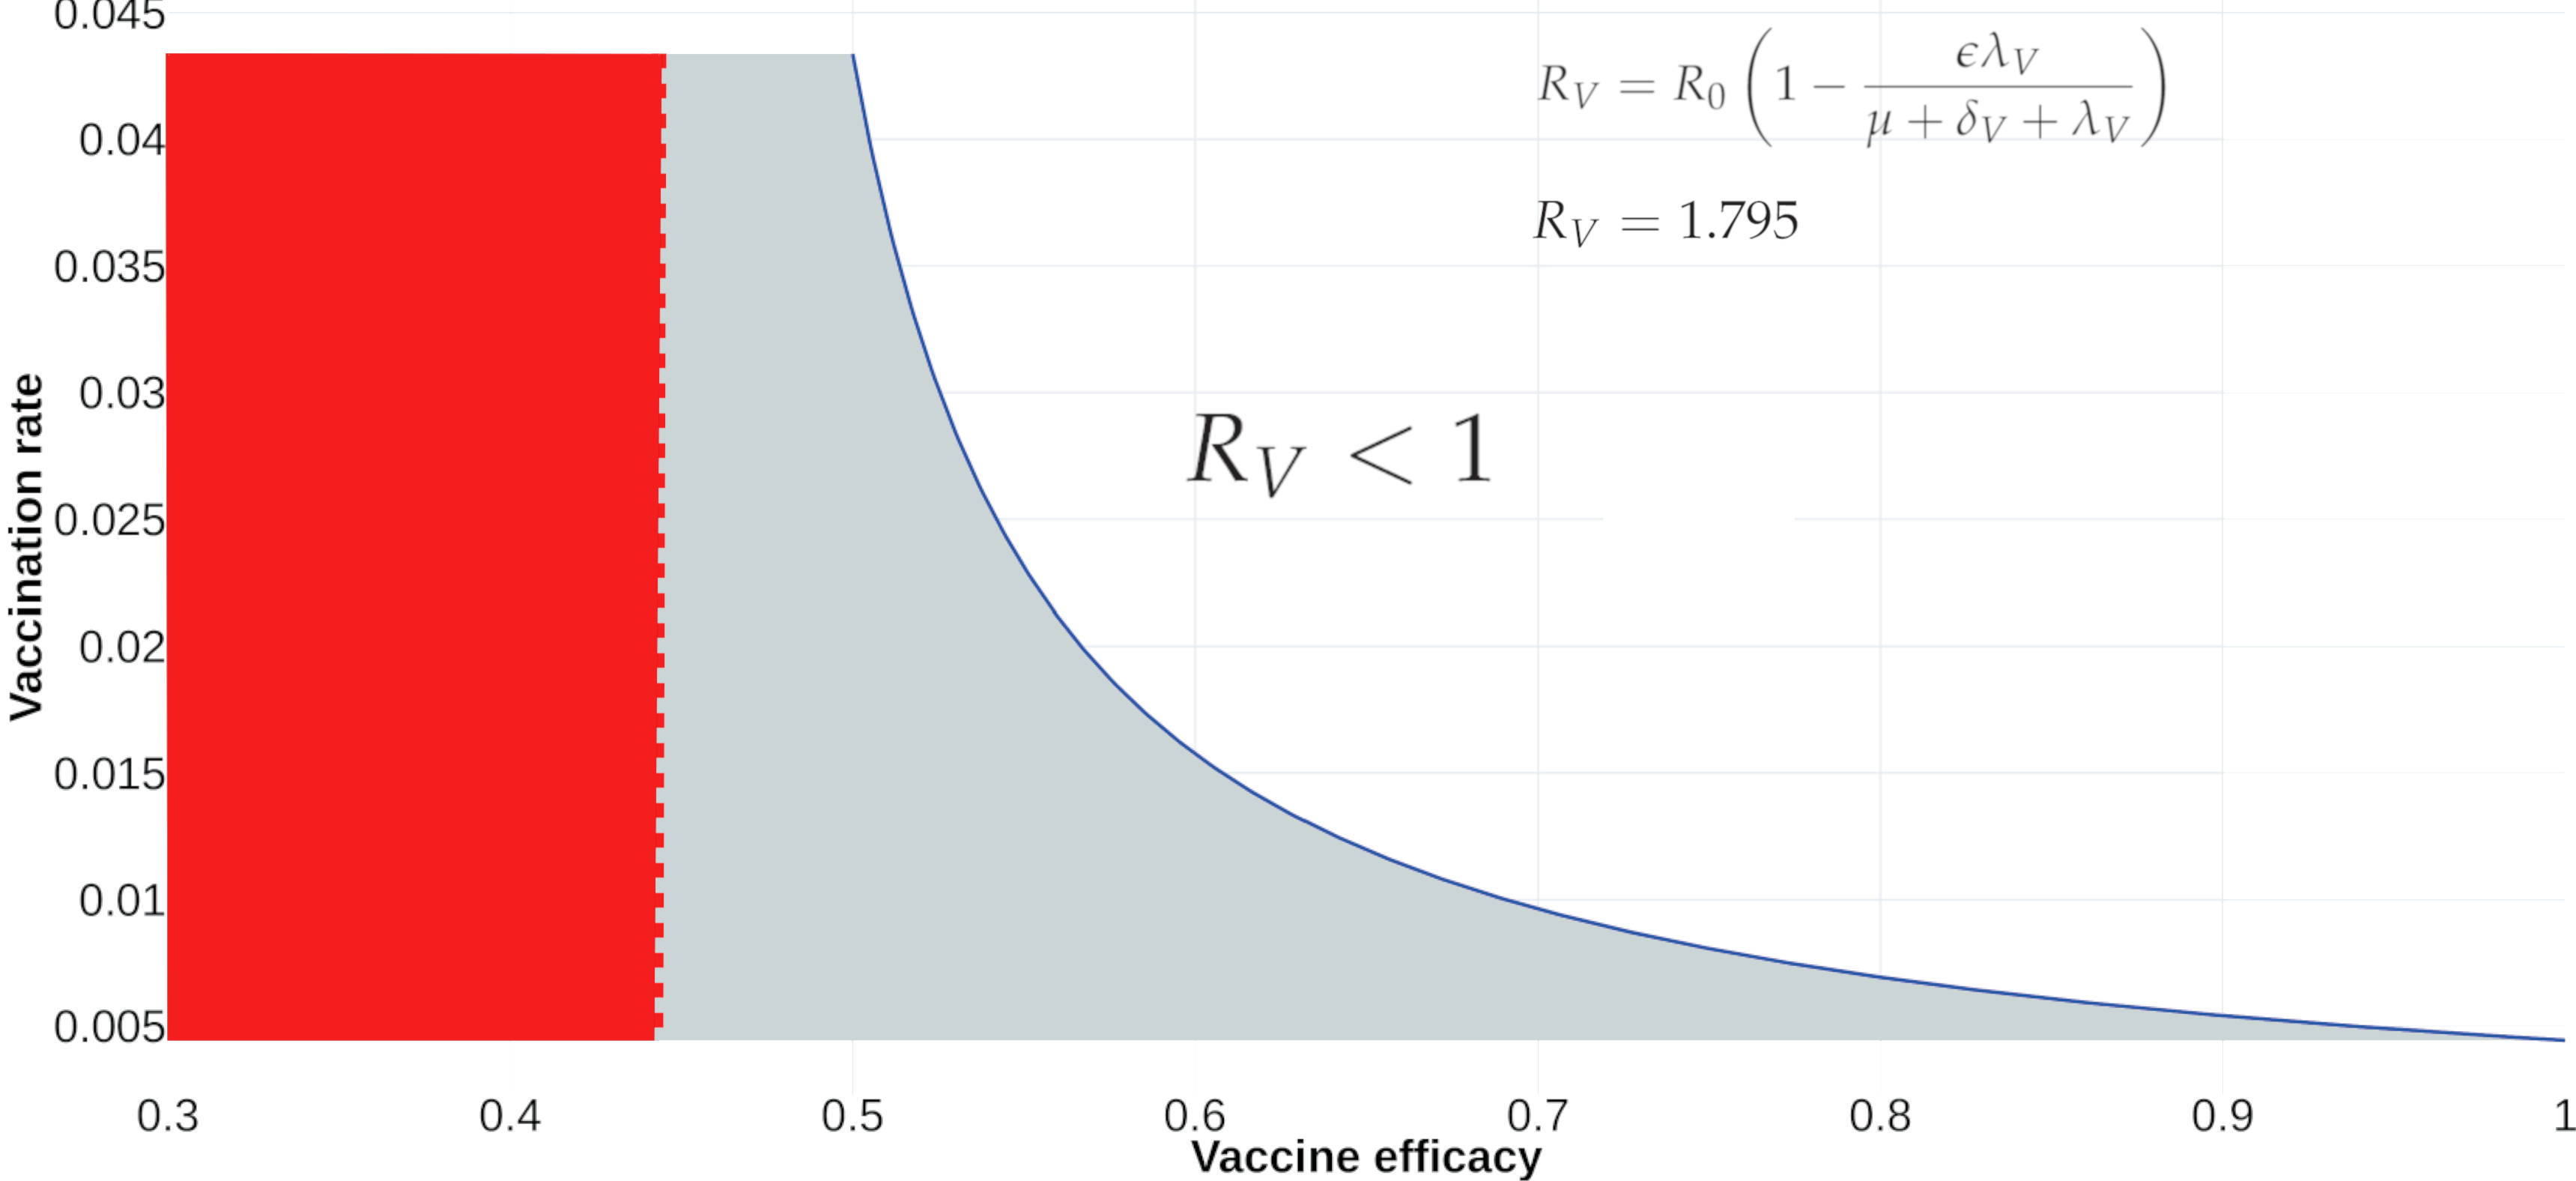
\includegraphics[scale=.875,%
            keepaspectratio]{assets/RvAnimation//r_zero_vac_efficiency04.png}
        }
        \only<5>{
            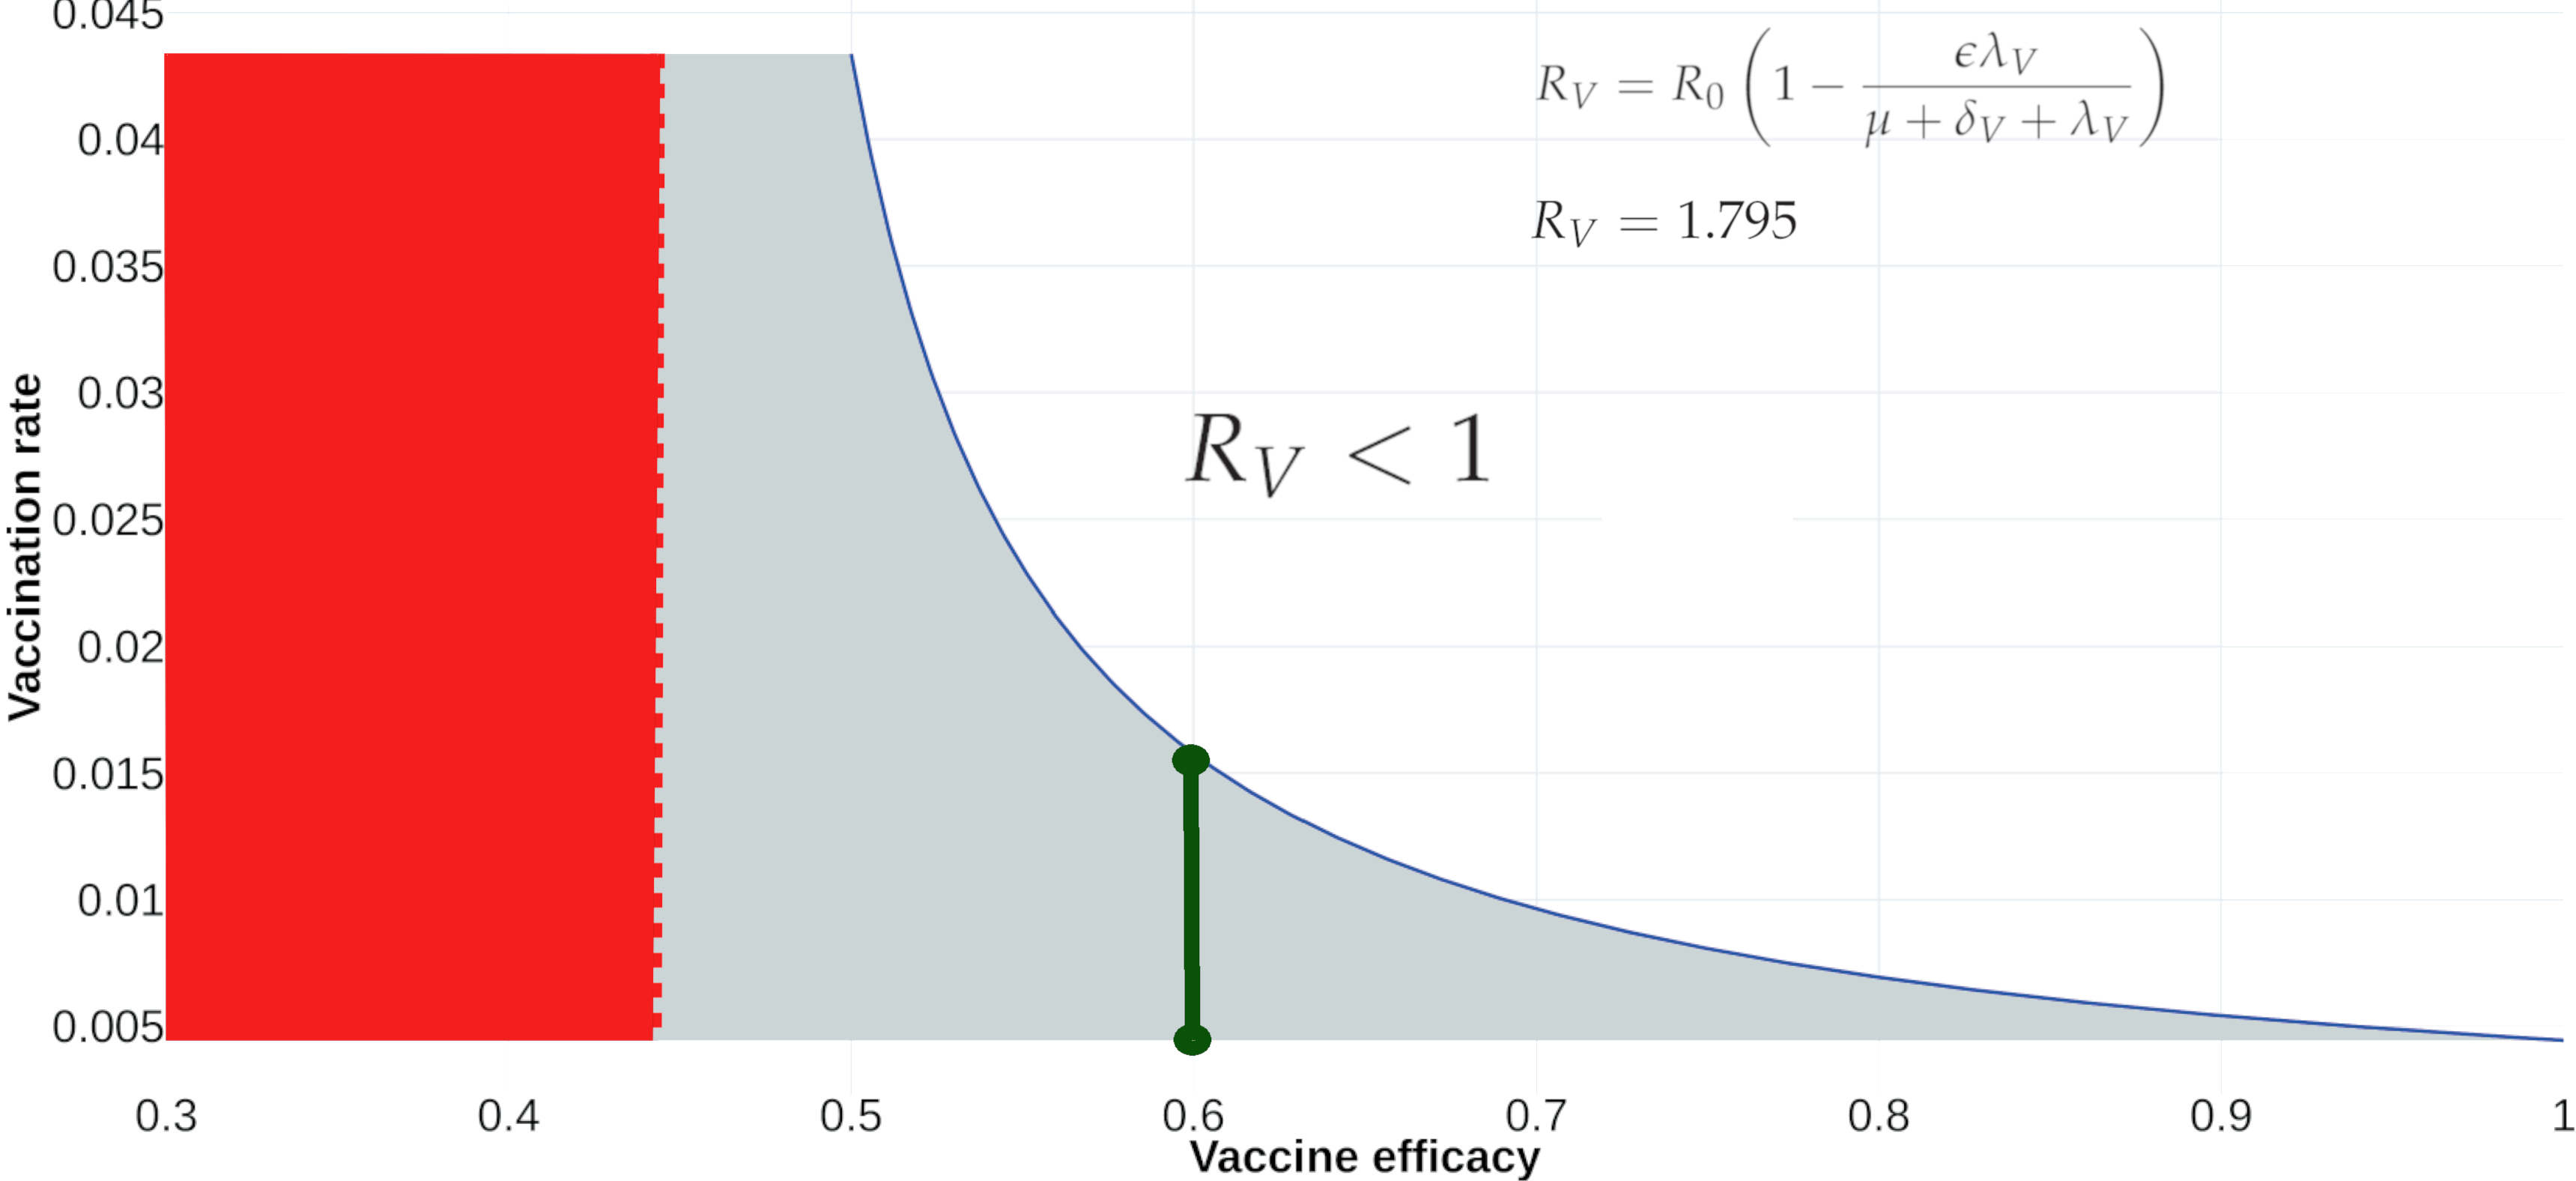
\includegraphics[scale=.875,%
            keepaspectratio]{assets/RvAnimation//r_zero_vac_efficiency05.png}
        }
        \only<6>{
            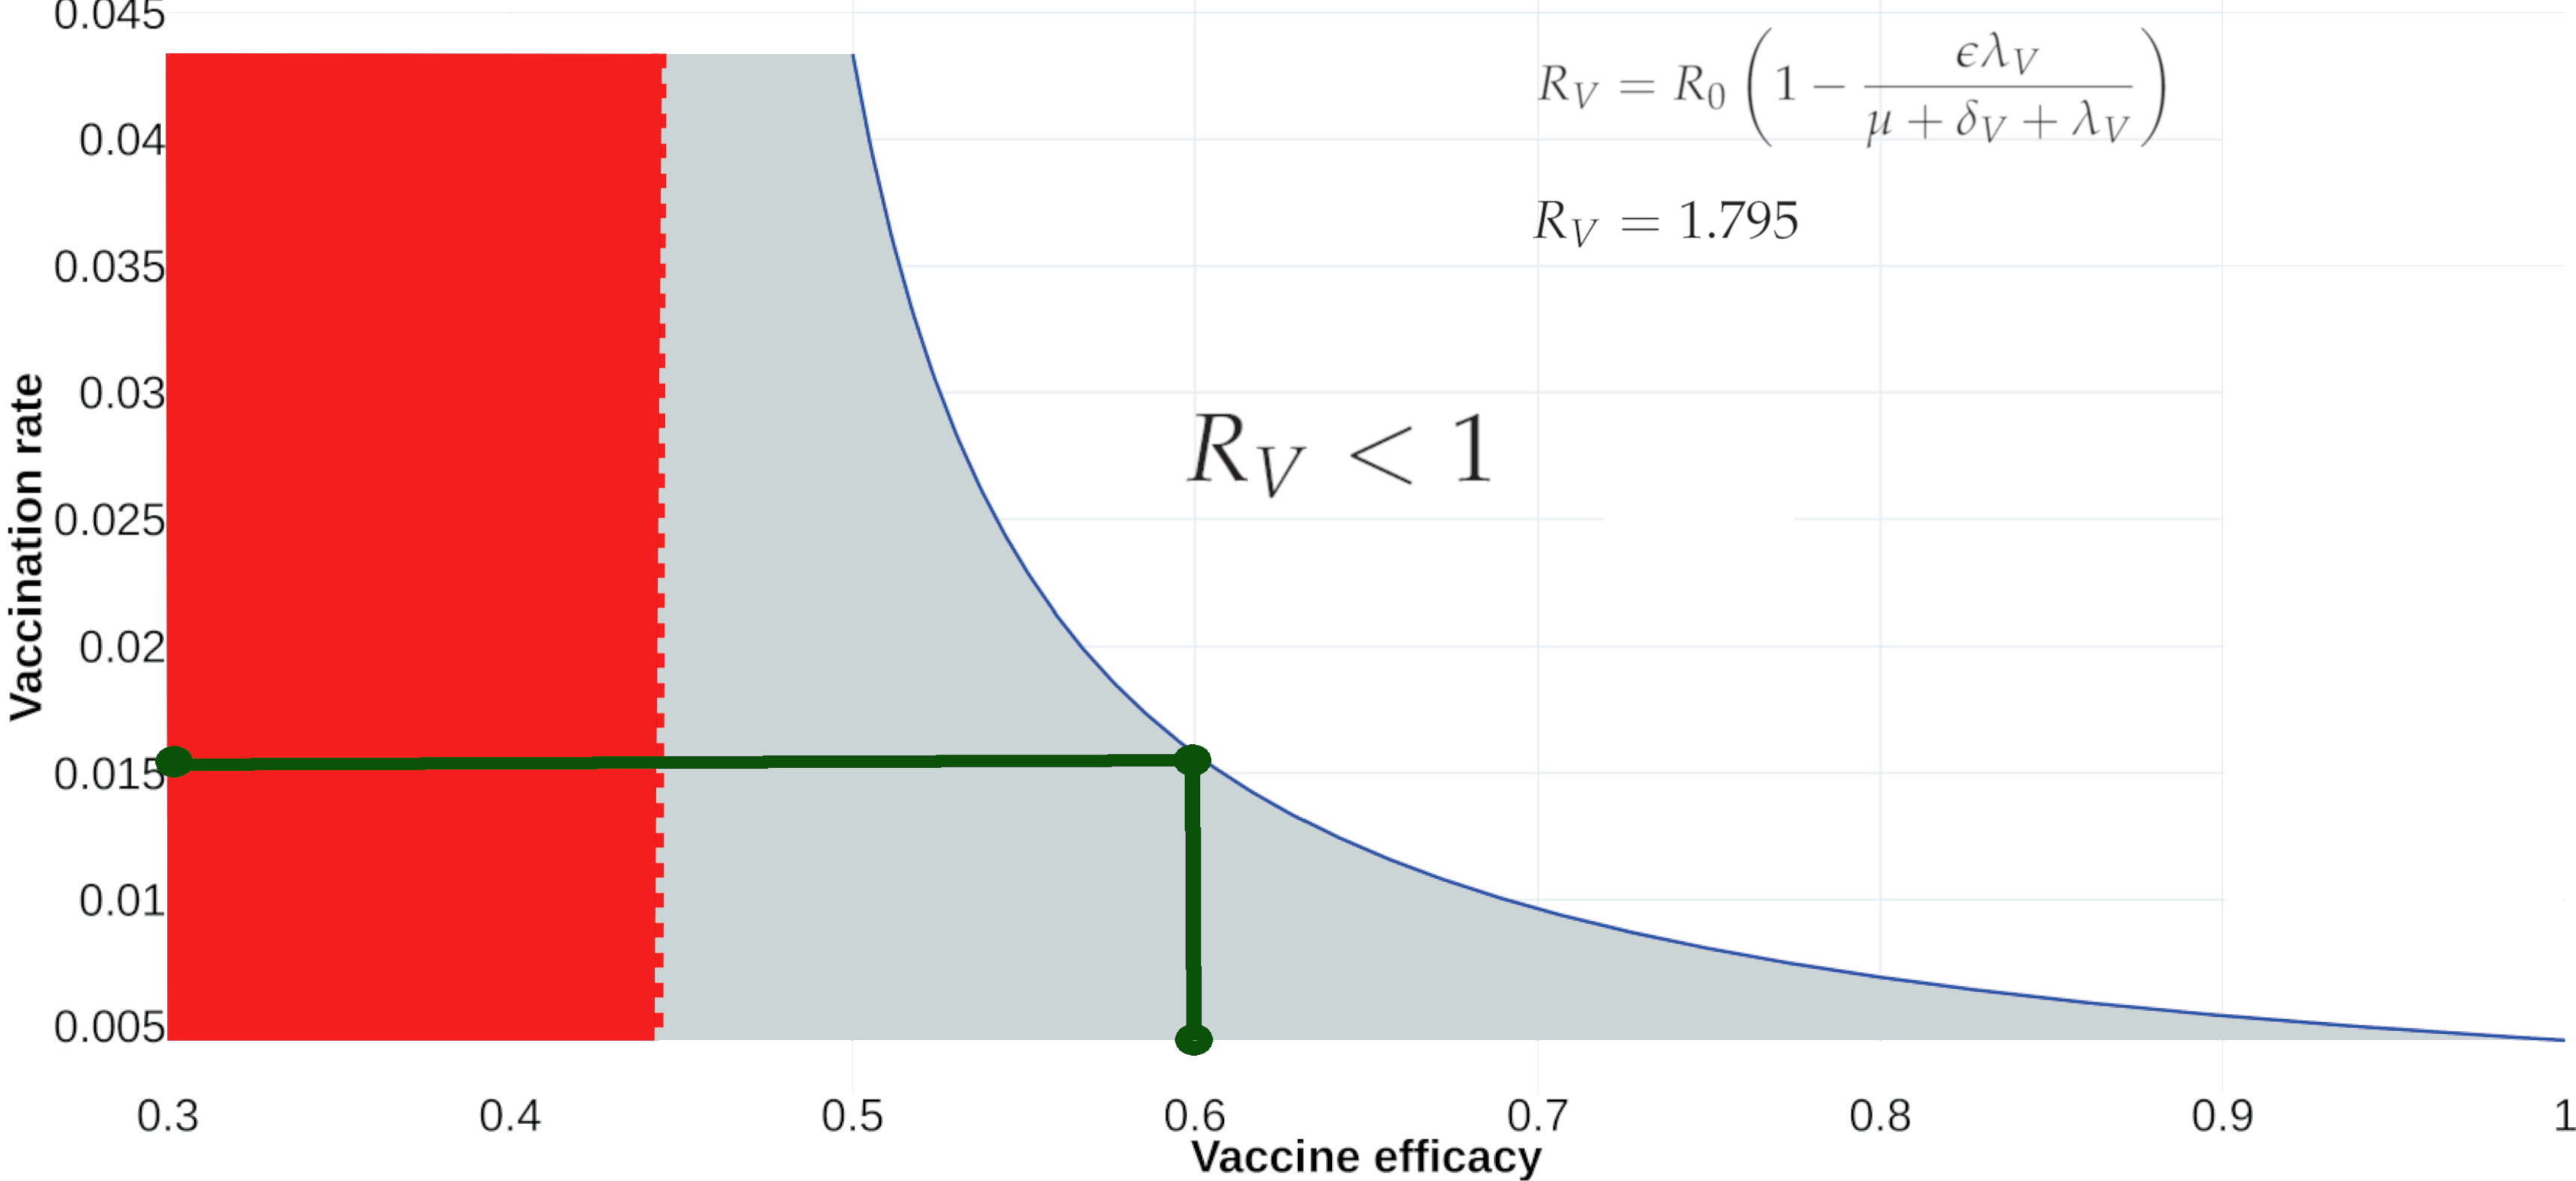
\includegraphics[scale=.875,%
            keepaspectratio]{assets/RvAnimation/r_zero_vac_efficiency06.png}
        }

    \end{textblock*}
%     \begin{textblock*}{120mm}(0mm, 10mm)
%         \only<7>{
%             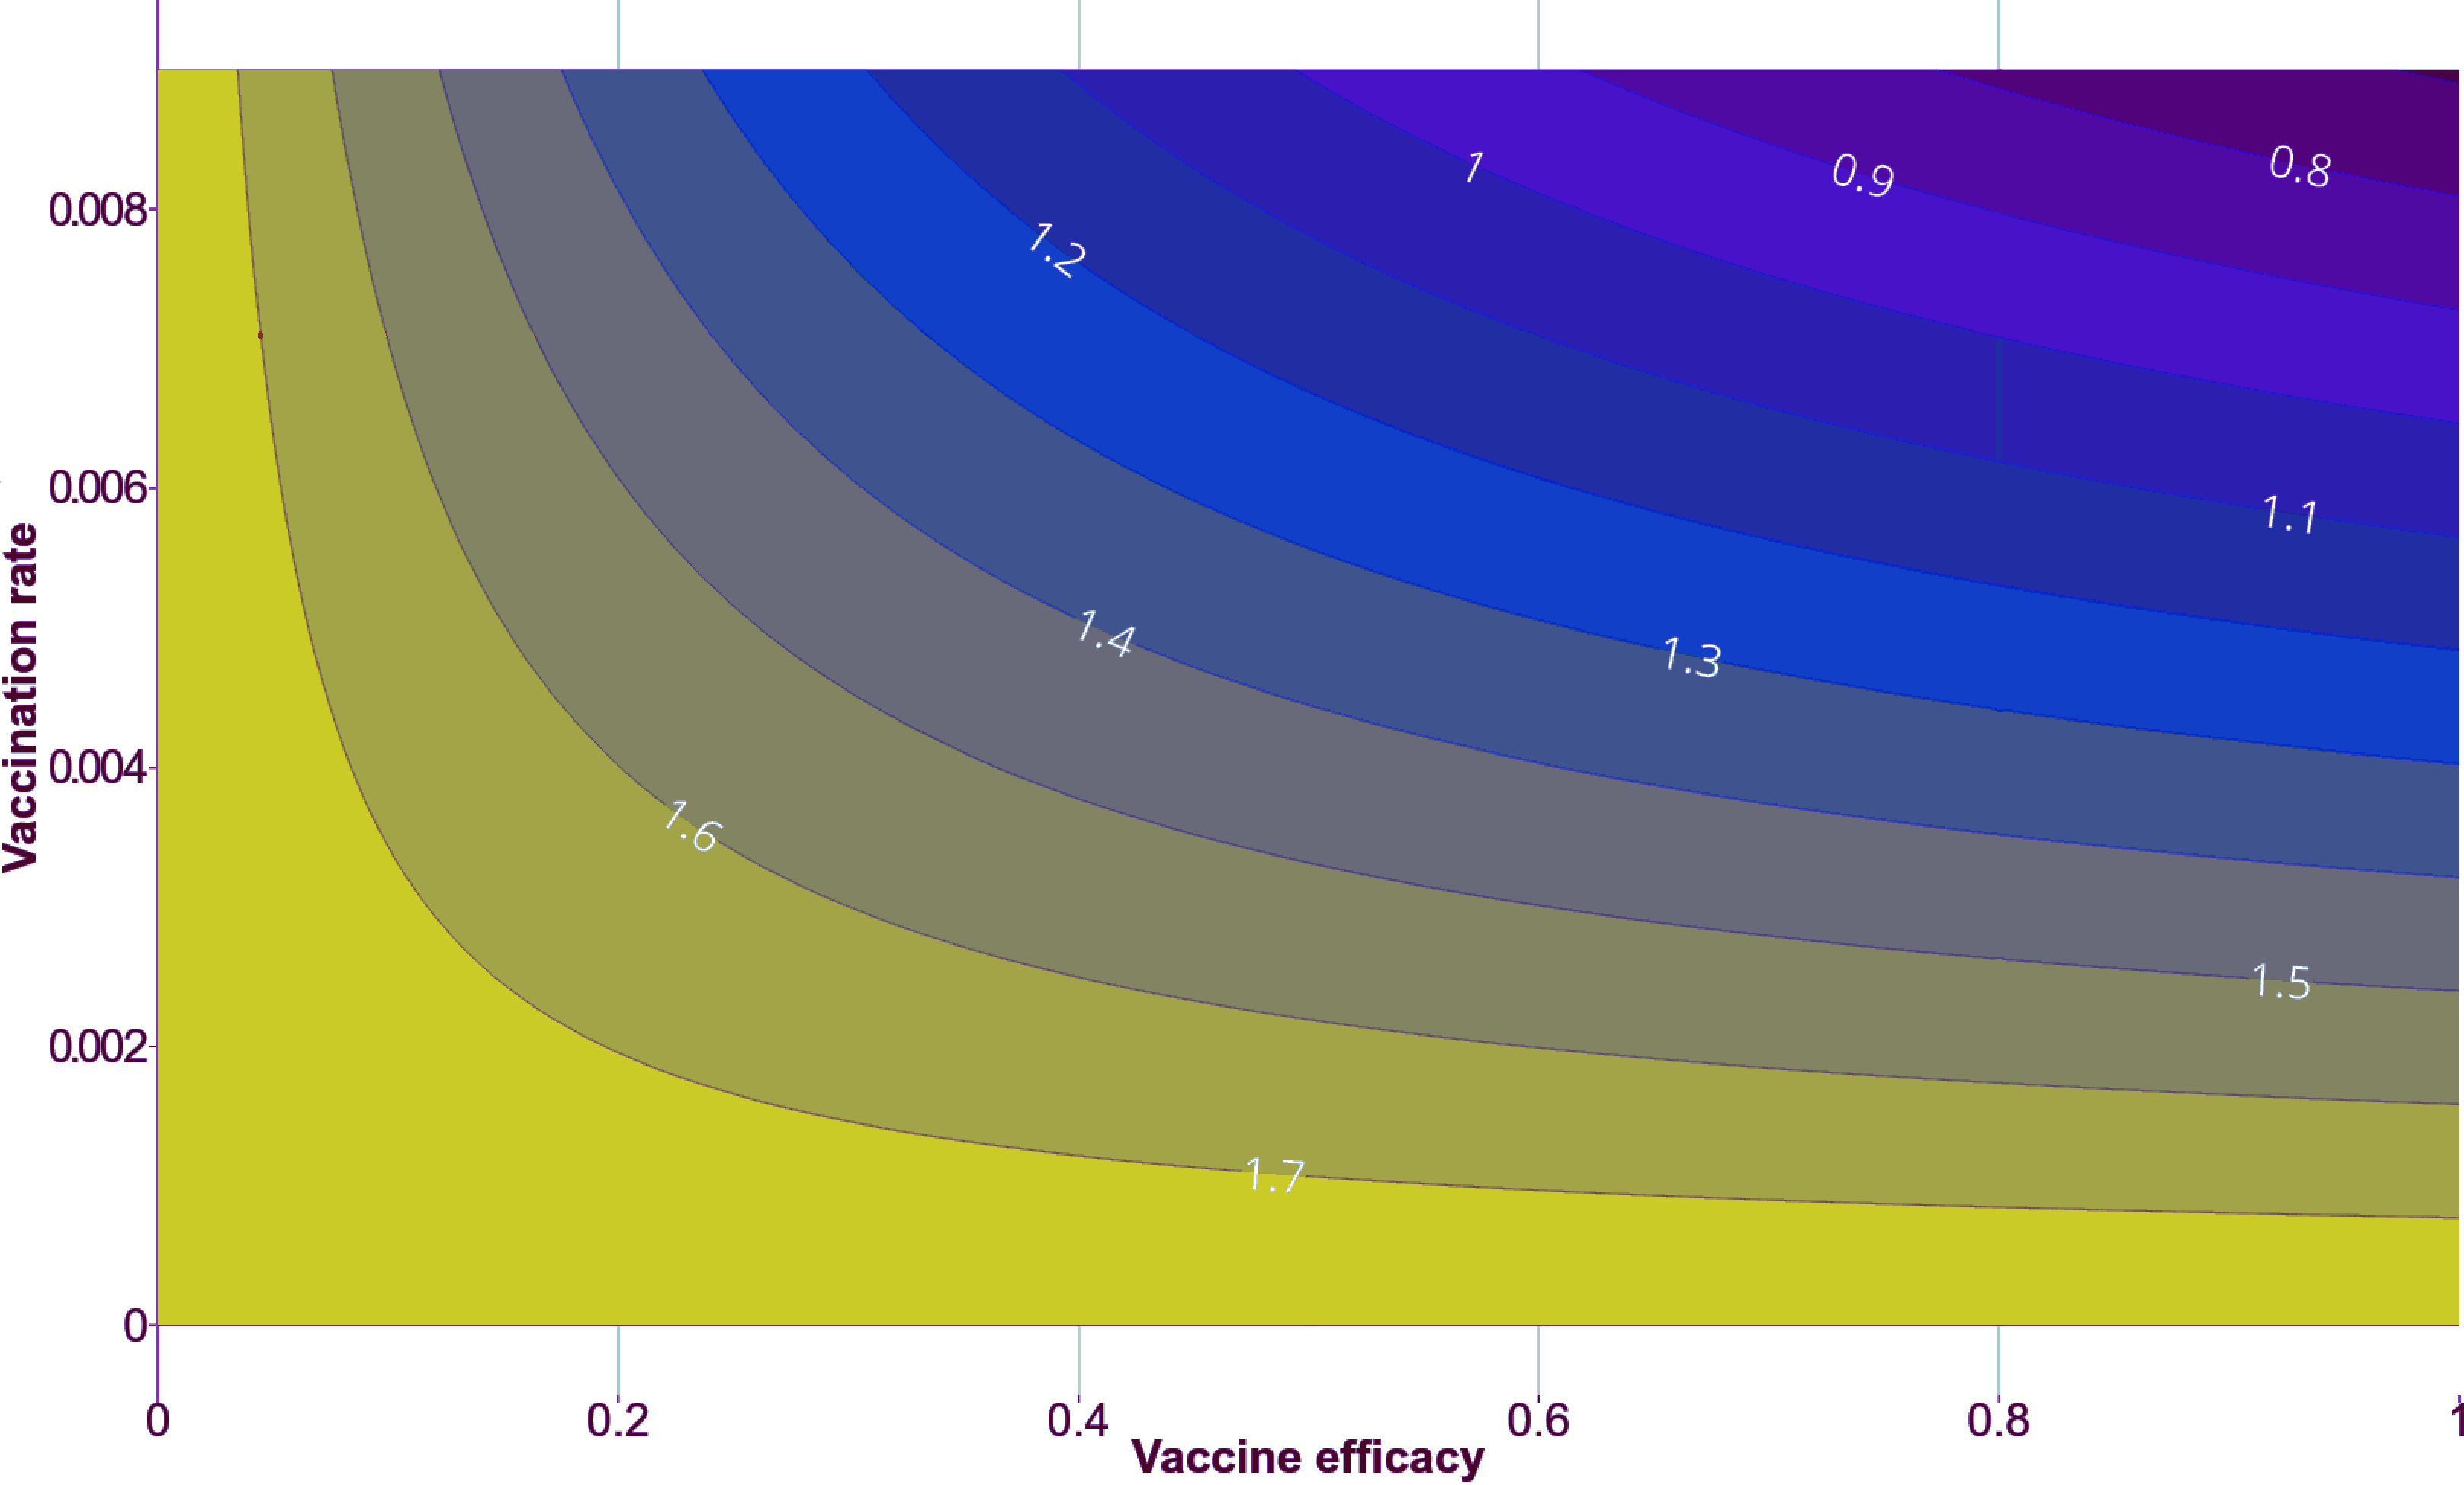
\includegraphics[scale=.65,%
%             keepaspectratio]{assets/RvAnimation/r_zero_vac_level_plots01.png}
%         }
%         \only<8>{
%             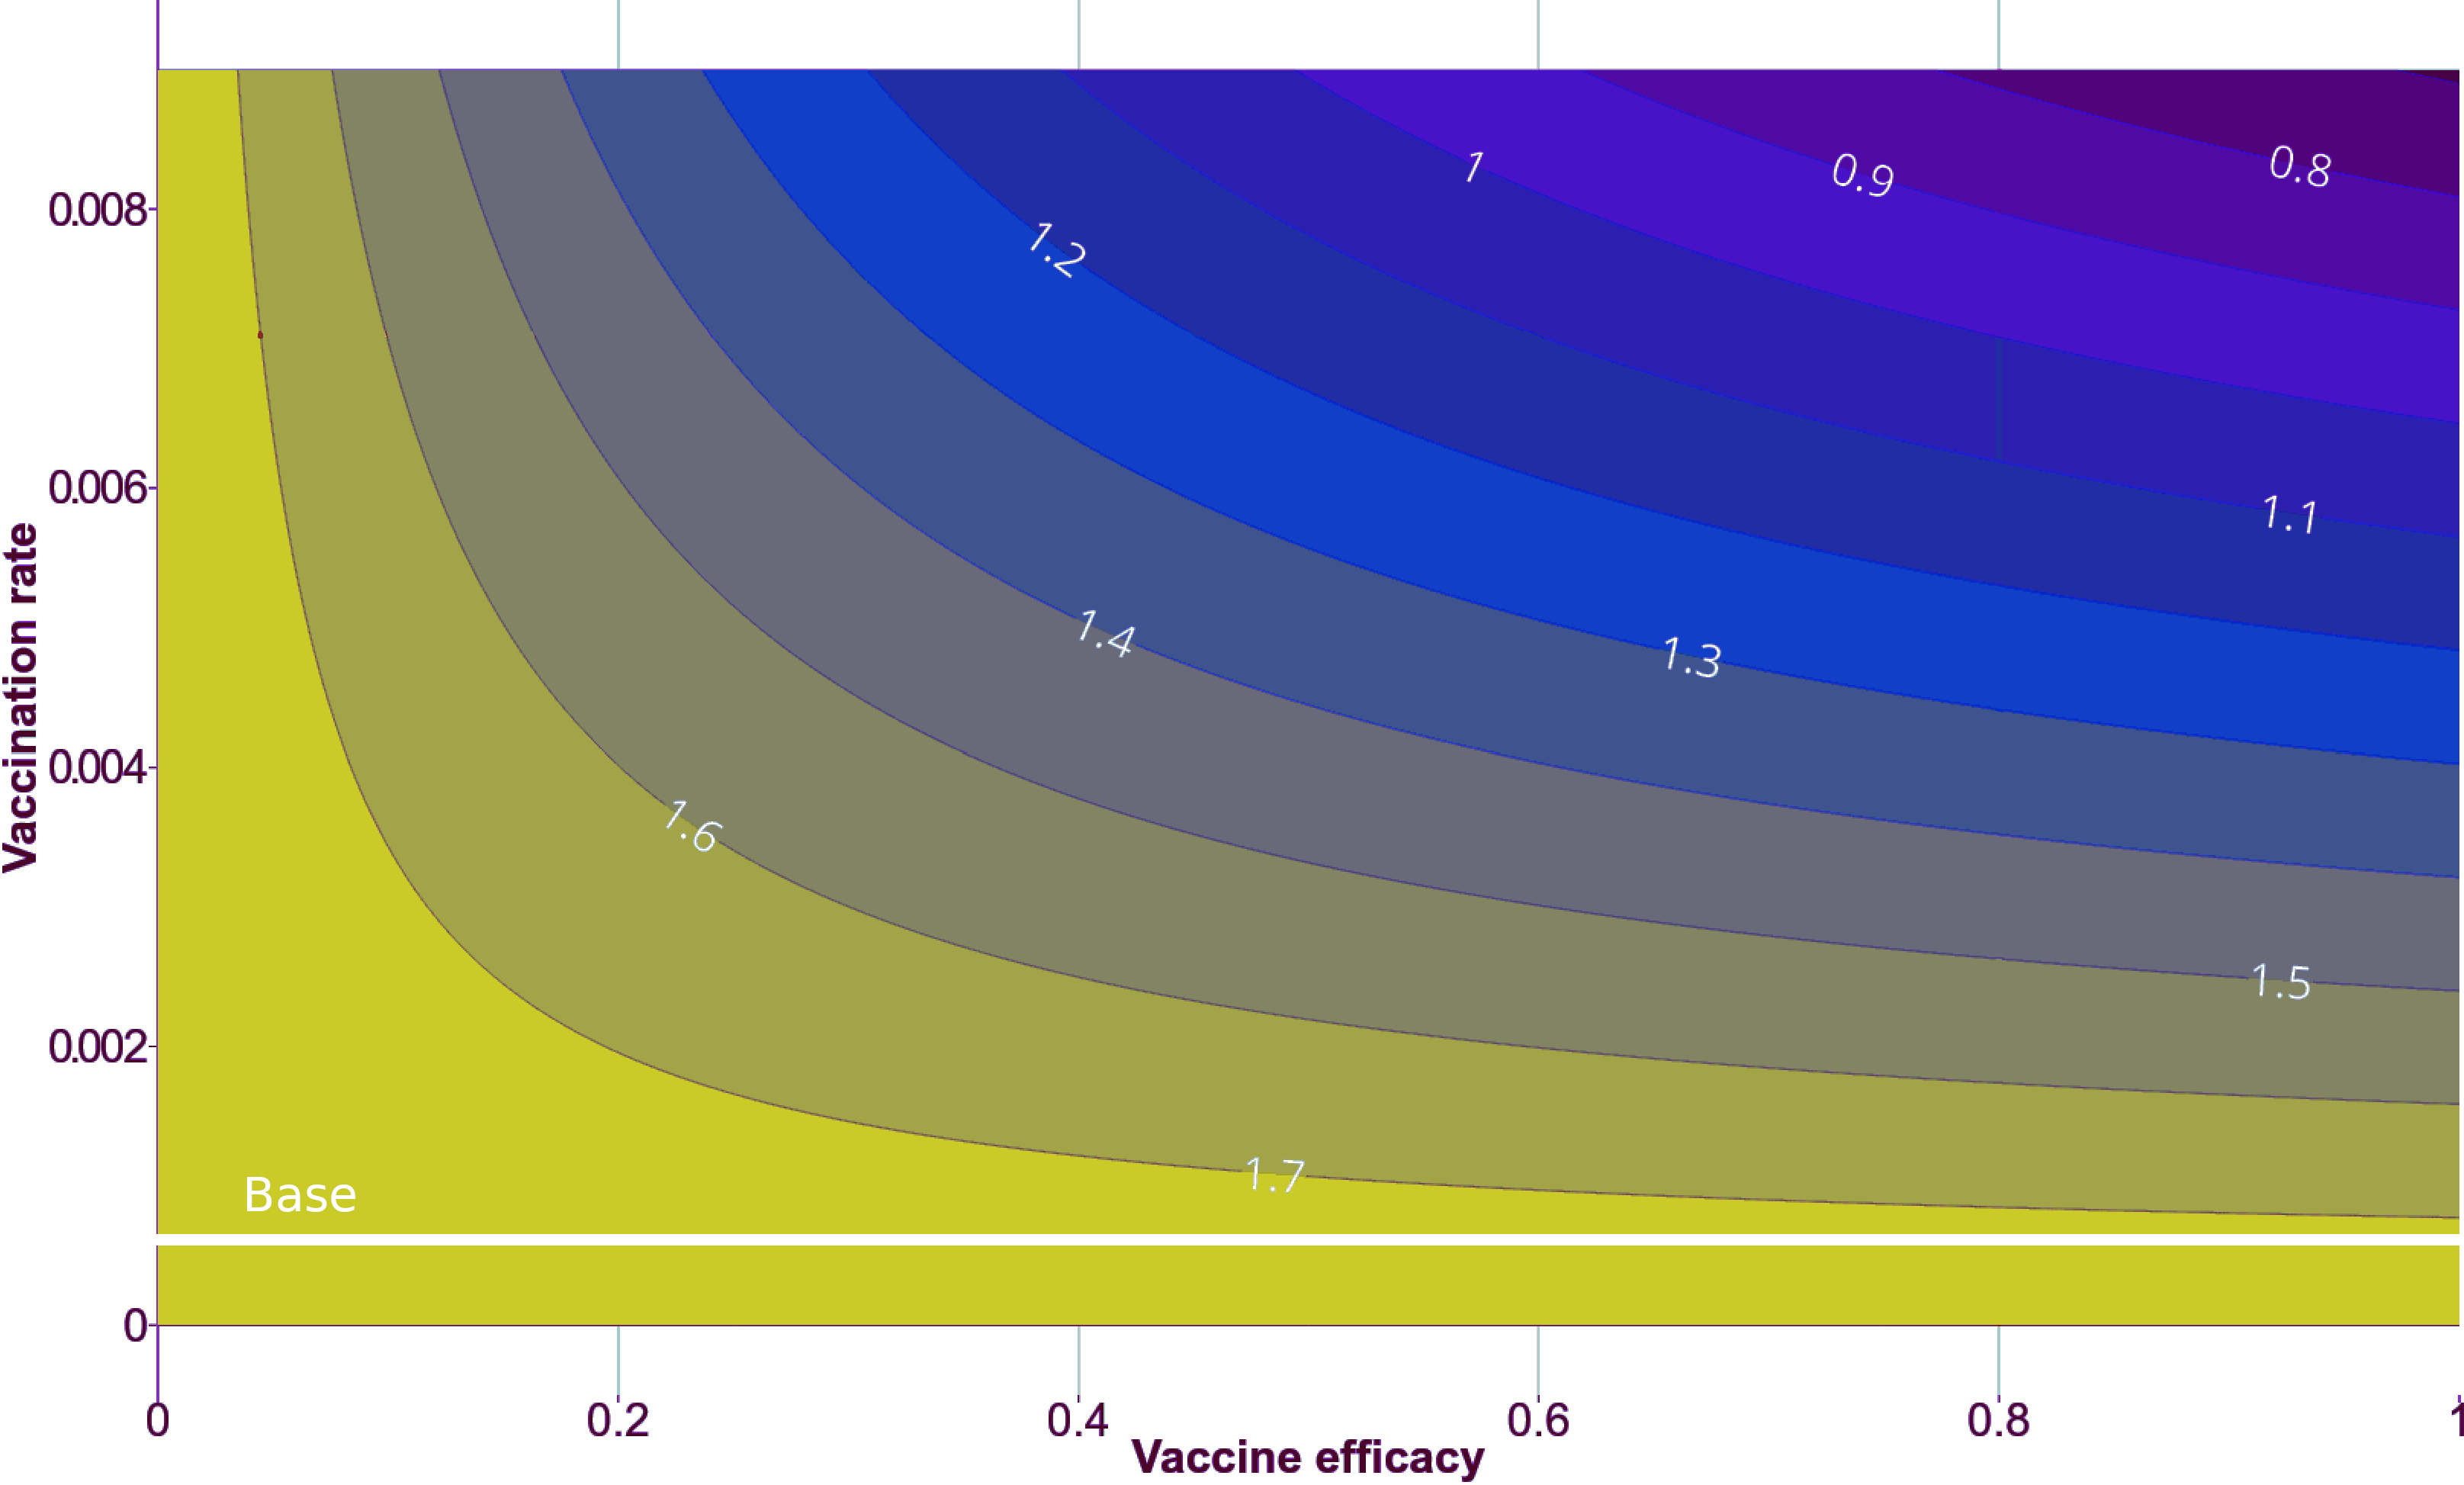
\includegraphics[scale=.65,%
%              keepaspectratio]{assets/RvAnimation/r_zero_vac_level_plots02.png}
%         }
%         \only<9>{
%             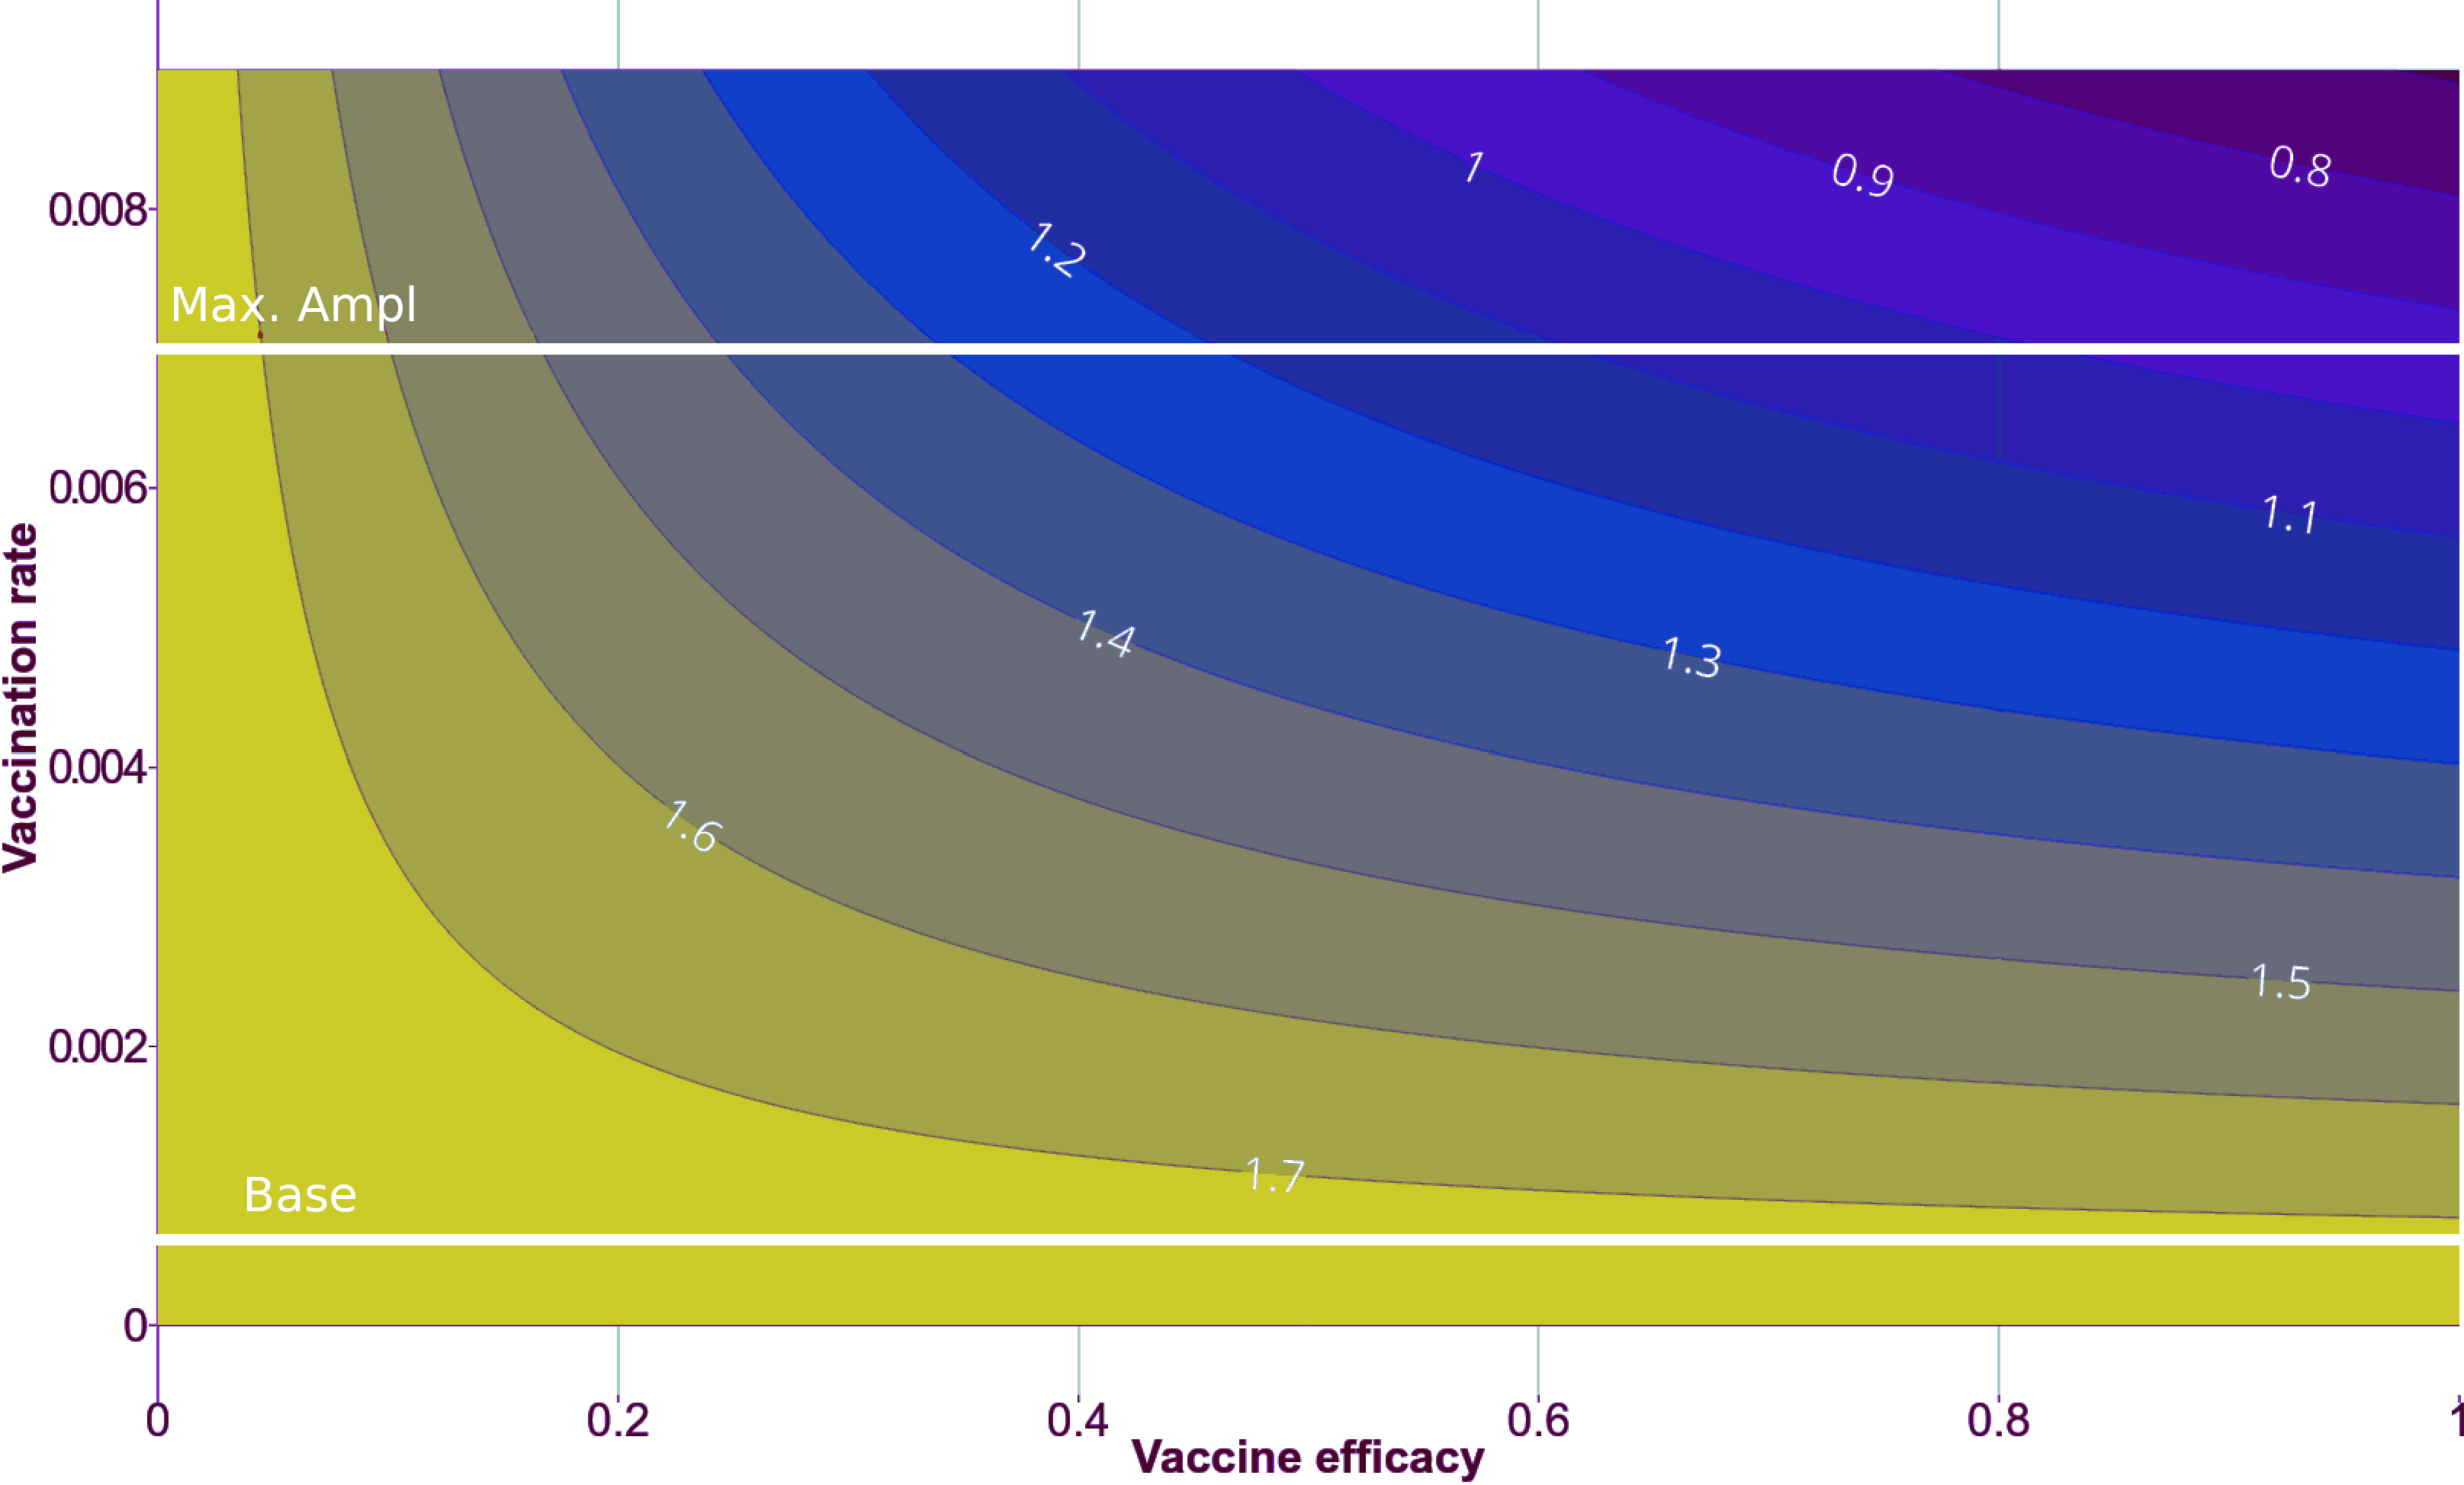
\includegraphics[scale=.65,%
%              keepaspectratio]{assets/RvAnimation/r_zero_vac_level_plots03.png}
%         }
%         \only<10>{
%             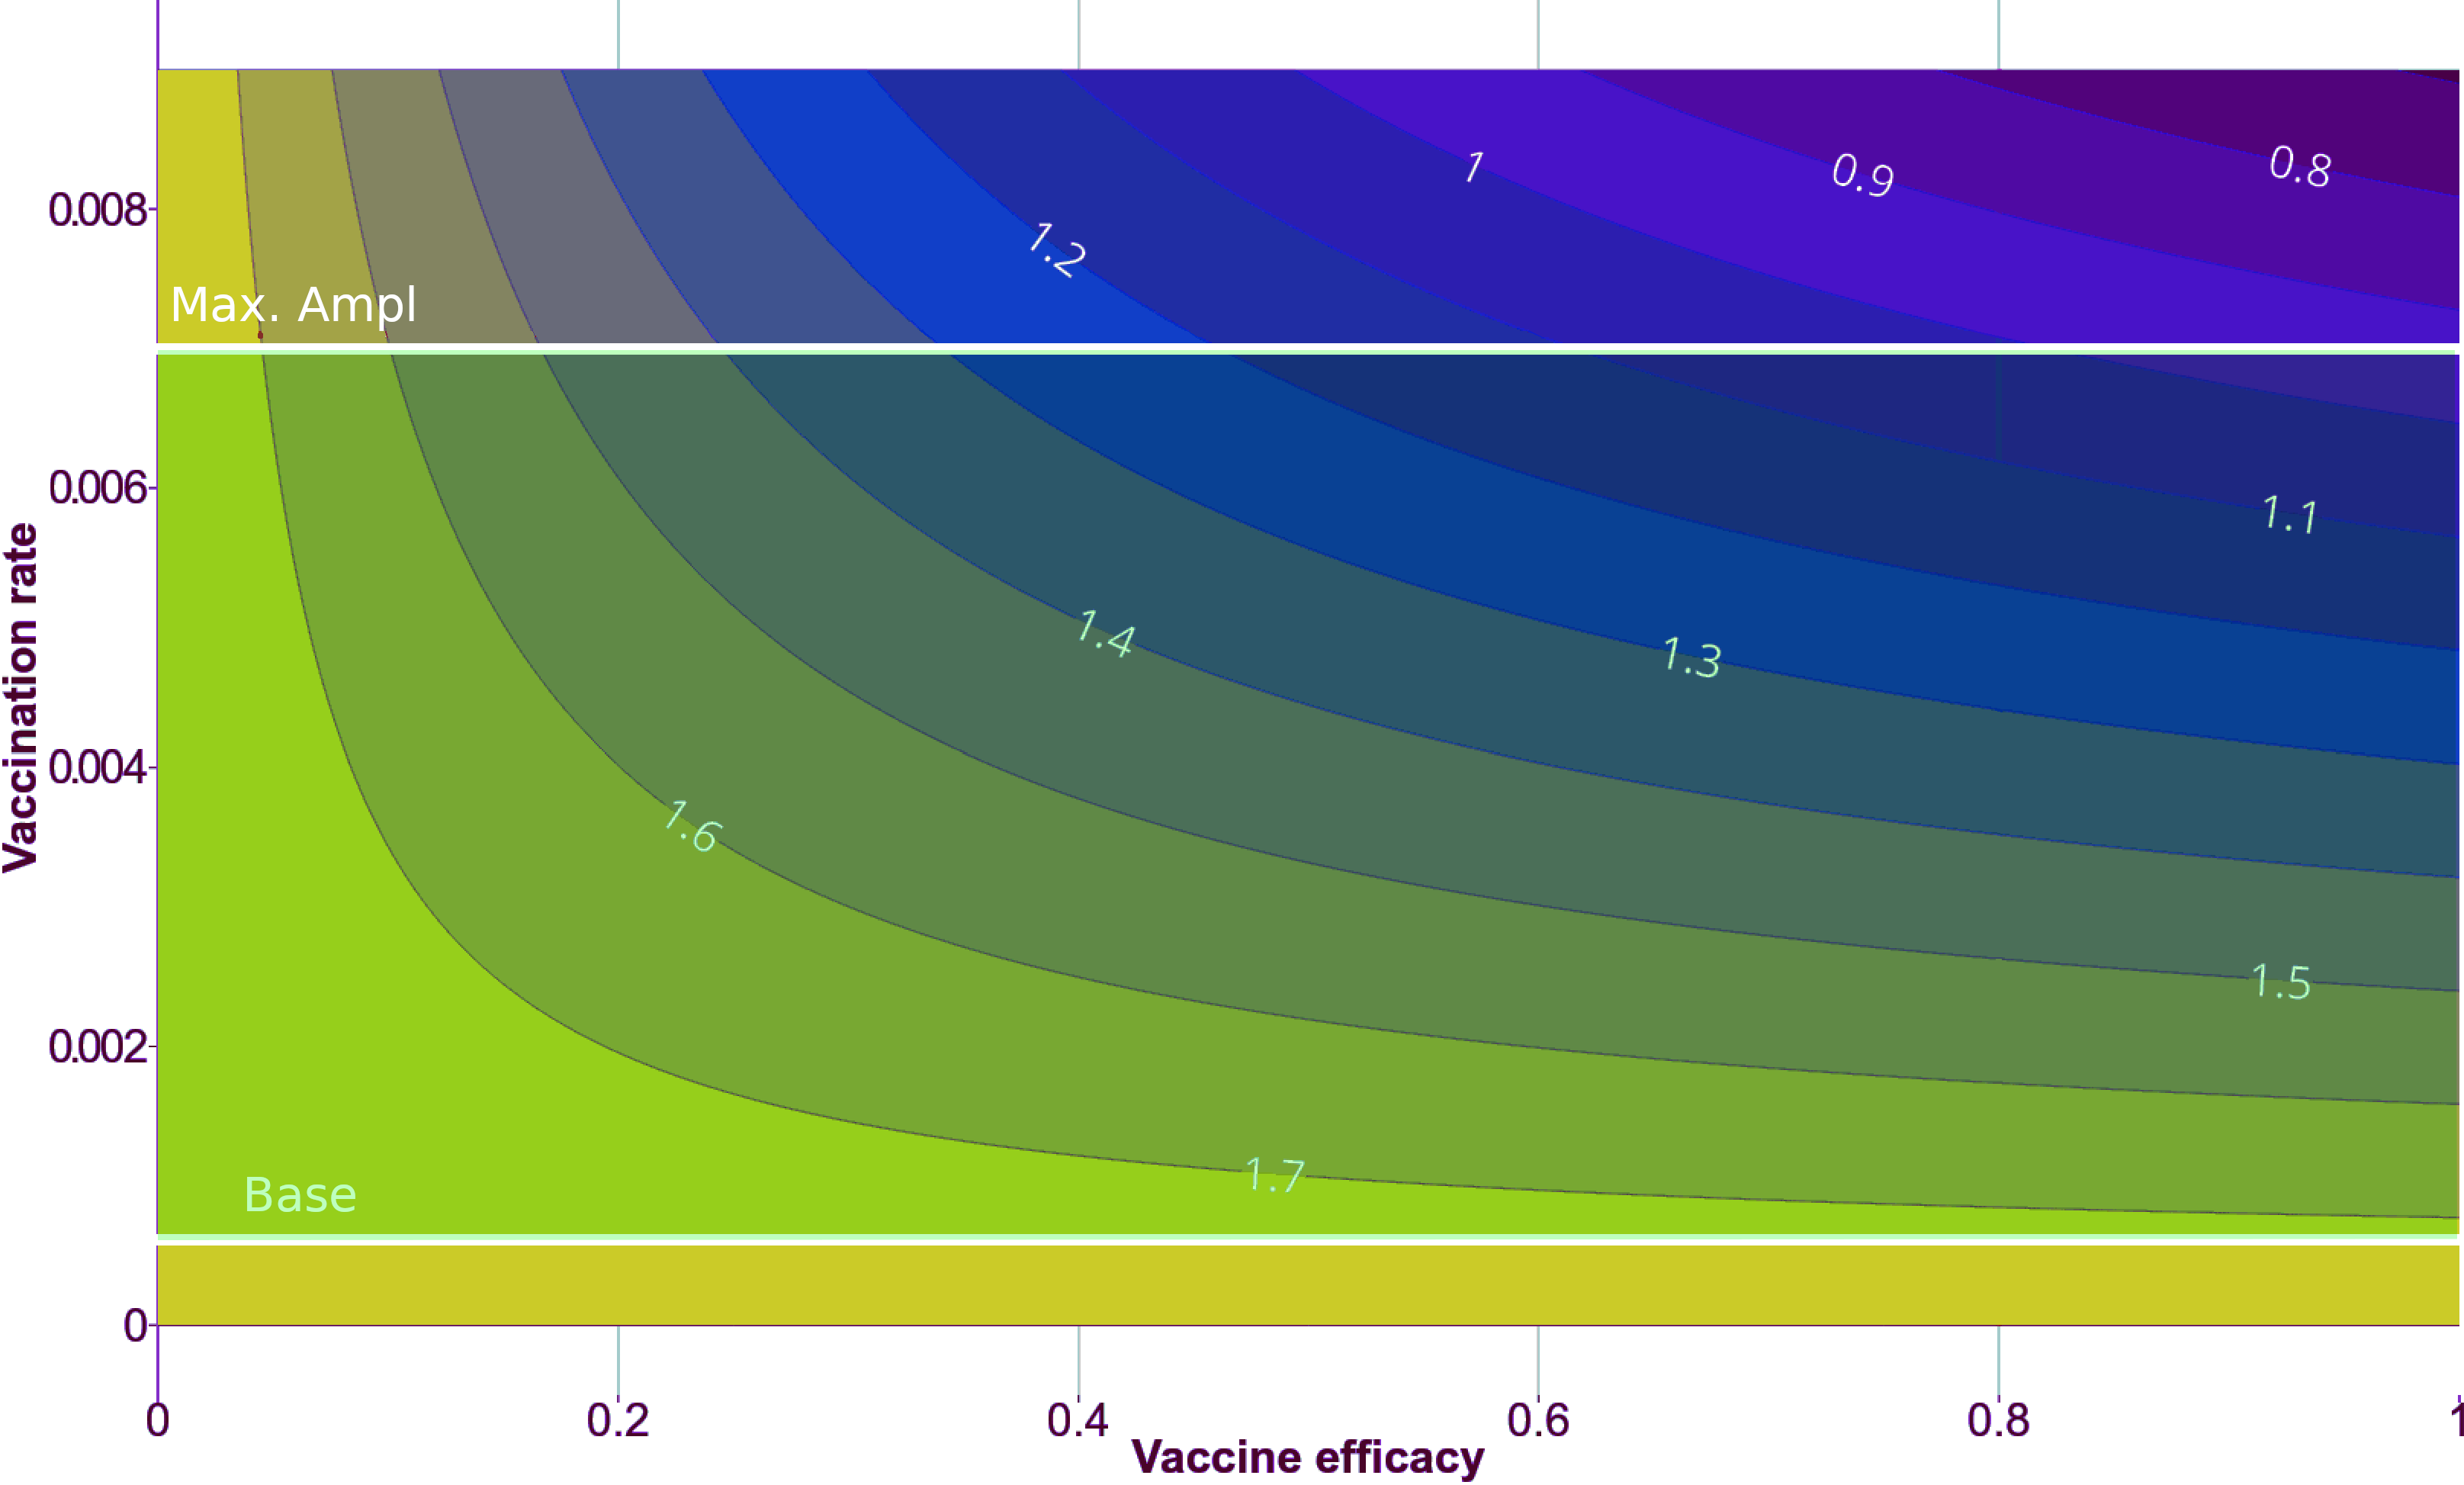
\includegraphics[scale=.65,%
%              keepaspectratio]{assets/RvAnimation/r_zero_vac_level_plots04.png}
%         }
%         \only<11>{
%             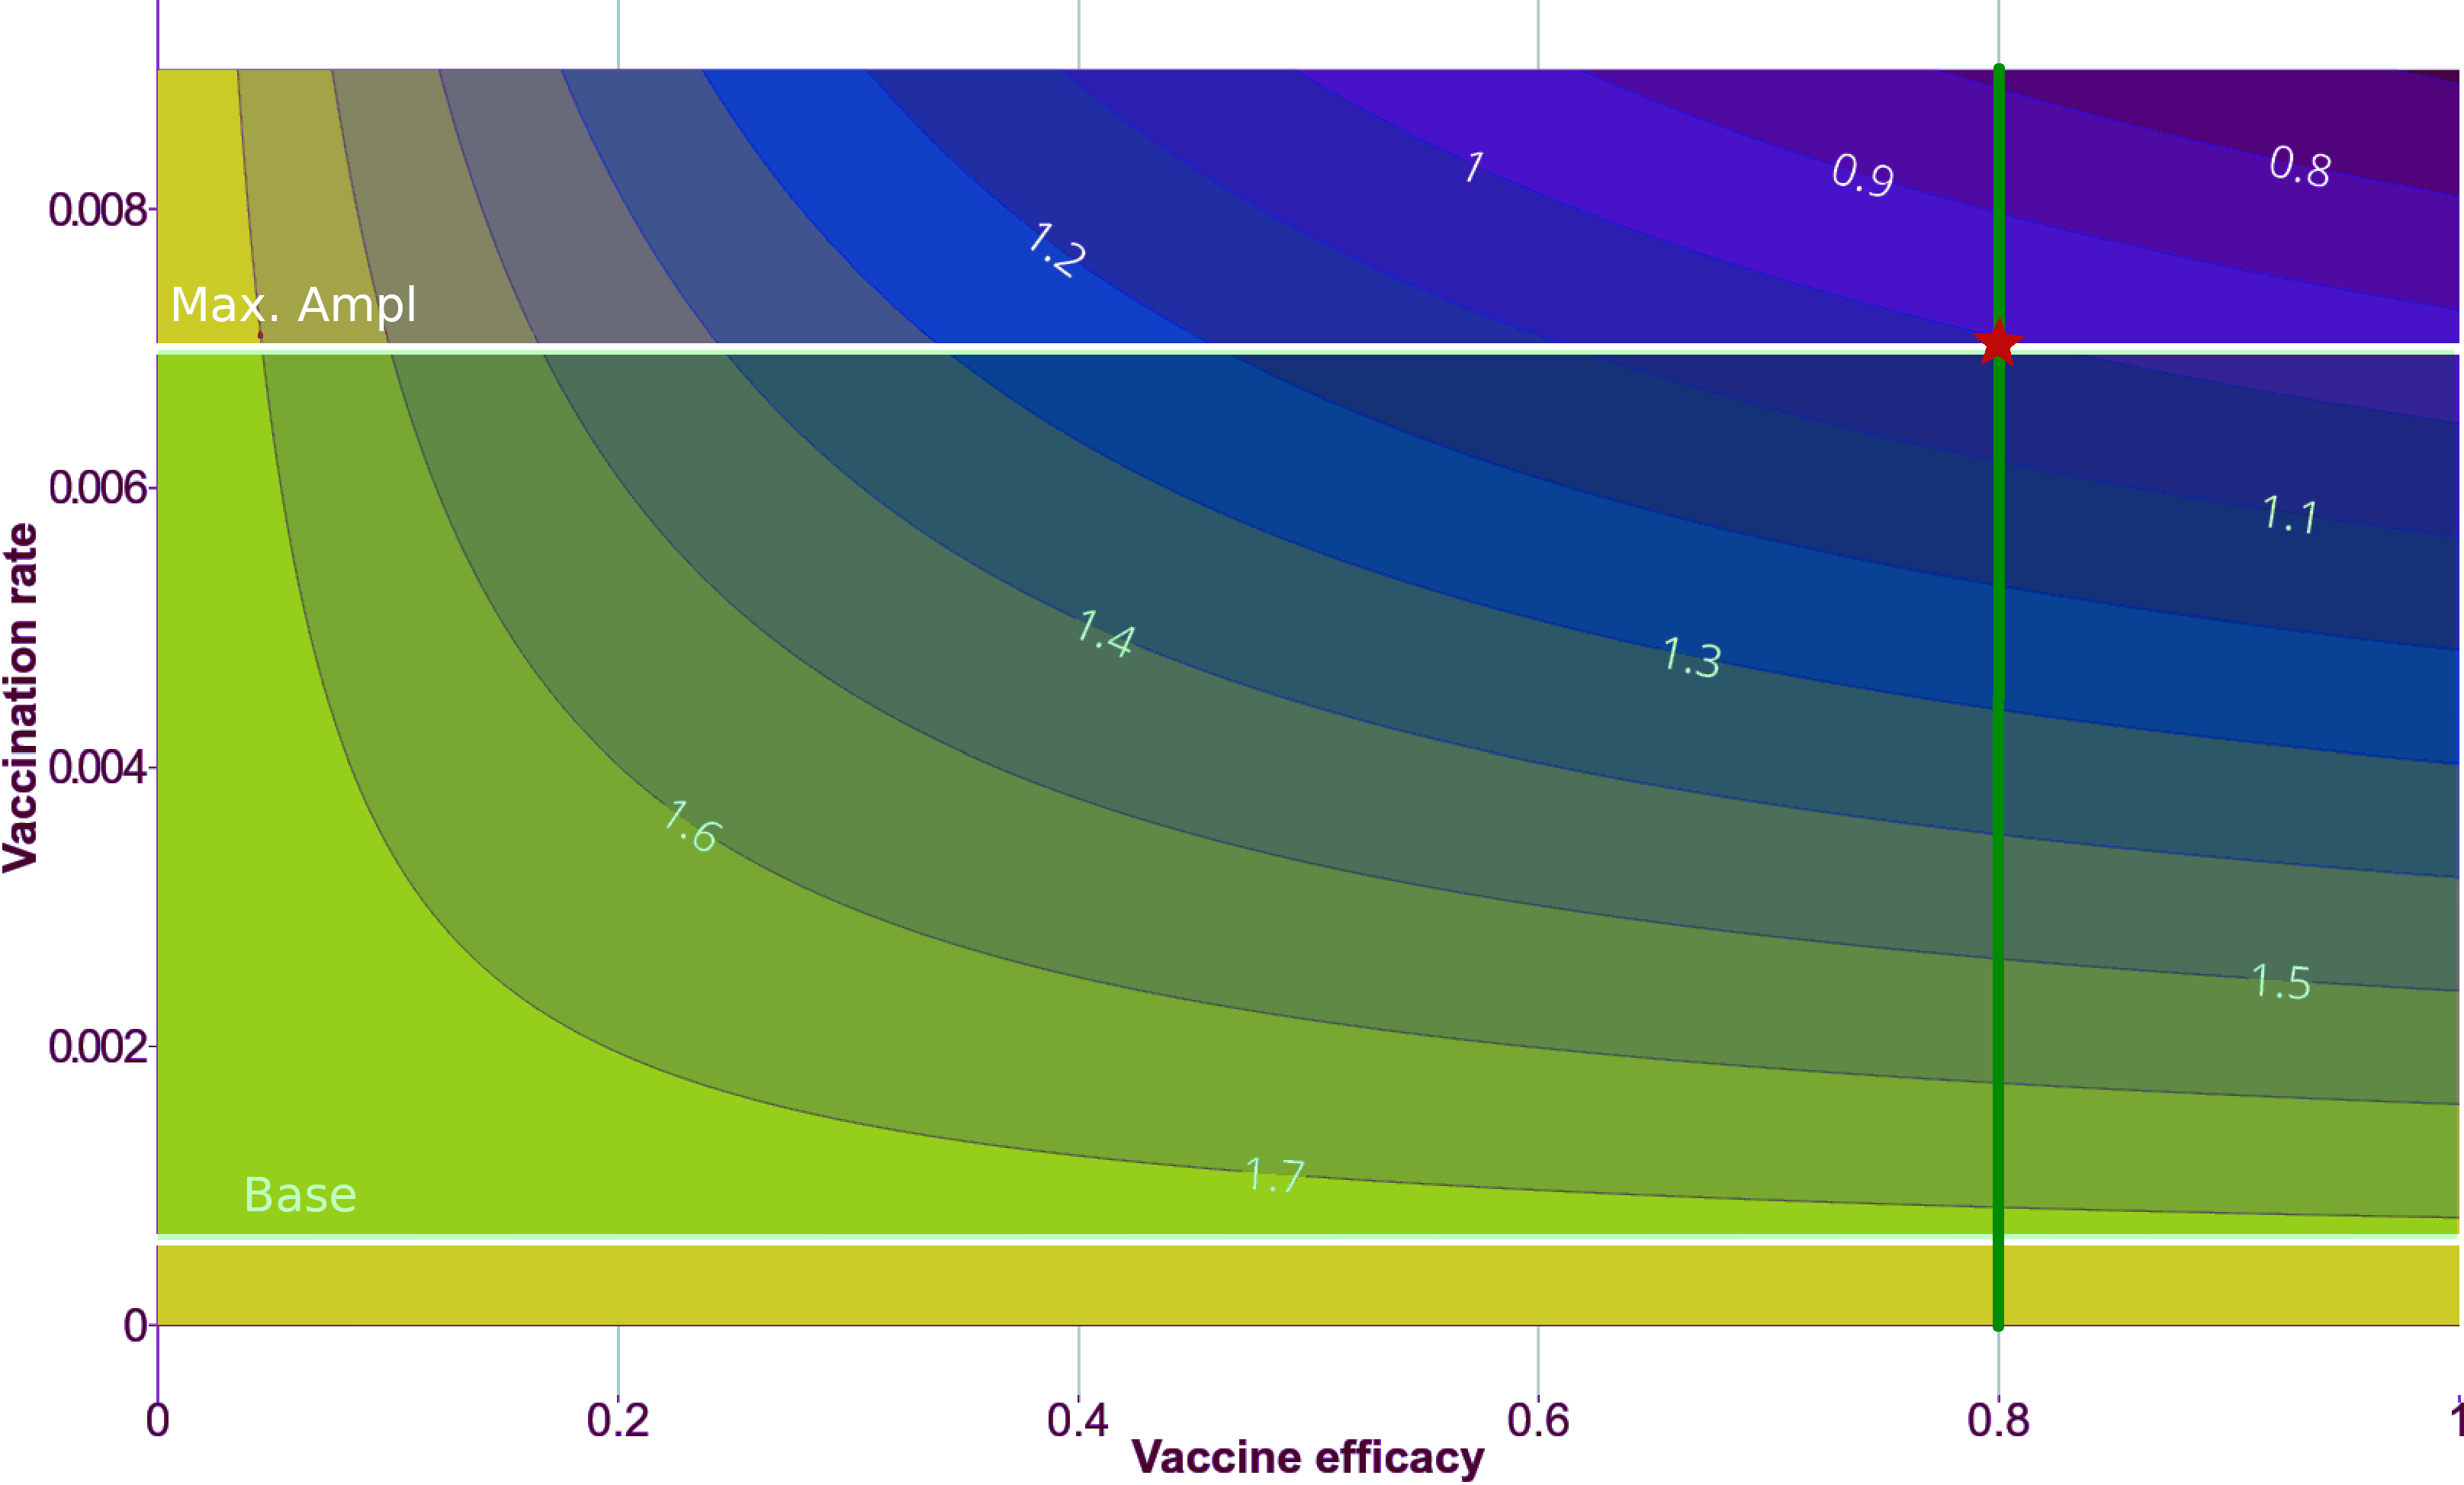
\includegraphics[scale=.65,%
%              keepaspectratio]{assets/RvAnimation/r_zero_vac_level_plots05.png}
%         }
%     \end{textblock*}
% %
%     \begin{textblock*}{40mm}(3mm, 65mm)
%         \only<8->{
%             \begin{graybox}{$\lambda_V$ estimation}
%                 Given a fixed coverage $X_{cov}$ and
%                 time horizon $T$
%                 $$
%                     1 - \exp(- \lambda_V T) = X_{cov}
%                 $$
%             \end{graybox}
%         }
%     \end{textblock*}
%     \begin{textblock*}{37mm}(90mm, 10mm)
%         \only<9->{
%             \begin{greenbox}{
%                 $X_{COV}: \SI{20}{\percent} \\
%                 T:\SI{1}{year}$
%         }
%         $
%             \lambda_V \approx 0.000611352
%         $
%         \tcblower
%         \only<10->{
%             \hspace*{-.5cm}
%             To decrease  {$R_V\leq 1$},
%             \\
%             \hspace*{-.5cm}
%             we require
%             $$
%                 \epsilon \geq 0.8, 
%                 \quad 
%                 \lambda_V 
%                 \geq \num{0.007}
%             $$
%         }
%            \end{greenbox}
%         }
%     \end{textblock*}
\end{frame}